\documentclass[10pt]{beamer}
\usepackage{pgfpages}
%\usepackage[backend=biber,citestyle=verbose, bibstyle=apa]{biblatex}
%\setbeameroption{show notes on second screen}
\usepackage[backend=biber, style=apa]{biblatex}
\addbibresource{main.bib}
\usetheme{metropolis}
%\addbibresource{demo.bib}
\usepackage{appendixnumberbeamer}
\usepackage{CJKutf8}
\usepackage{tipa}
\usepackage{amsmath}
\usepackage{xfrac}
\usepackage{bm}
\usepackage{suffix}
\usepackage{amssymb}
\usepackage{braket}
\usepackage{physics}
\usepackage{amsthm}
\usepackage{mathtools}
\usepackage{booktabs}
\usepackage{scalerel}
\usepackage[scale=2]{ccicons}
\usepackage{pgfplots}
\usepackage{subcaption}
\usepackage{algorithm}
\usepackage[noend]{algpseudocode} 
\usepackage{graphicx}
\usepackage{tikz}
\usepackage{mdframed}
\usepgfplotslibrary{dateplot}
%\let\footcite\footfullcite
\usepackage{xspace}
\usepackage{verbatim}
\newcommand{\themename}{\textbf{\textsc{metropolis}}\xspace}

\title{基于 Pauli 路径积分模拟量子线路}
\date{May 8, 2025}
\author{答辩人:邵钰果\\
导师:刘正伟 教授}
\institute{Tsinghua University}
% \titlegraphic{\hfill\includegraphics[height=1.5cm]{logo.pdf}}

\begin{document}
\begin{CJK}{UTF8}{gbsn}
\maketitle
\note{Good afternoon. Thanks for the introduction.

It's a pleasure for a phd student to be here today.
If there is anything I have not done well, I sincerely(\textipa{sɪnˈsɪrli}) ask for your understanding and constructive feedback.

Today I will introduce our recent work about Pauli path Integral simulation for Noisy variational quantum circuits.}

\begin{frame}{Table of contents}
  \setbeamertemplate{section in toc}[sections numbered]
  \tableofcontents[hideallsubsections]
\end{frame}
\note{In this talk, I will first introduce the background of quantum computing and the quantum supermacy in noisy intermediate-scale quantum (NISQ) era. 
  
 Then, I will discuss the potential of variational quantum algorithms, which are useful for solving practical problems and designed for NISQ devices.
  
 Finally, I will introduce our recent work on the simulation of noisy variational quantum circuits.
  
 Let's get started.}

\section{Introduction}
\begin{frame}[fragile]{Moore’s law}
  \begin{minipage}{0.23\textwidth}
    \begin{figure}
      \centering
      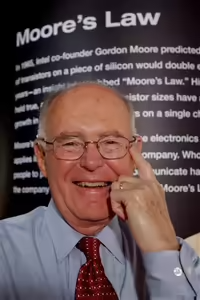
\includegraphics[width=\textwidth]{fig/moore0.png}
    \end{figure}
  \end{minipage}
  \begin{minipage}{0.75\textwidth}
    \vspace{3em}
    \begin{figure}
      \centering
      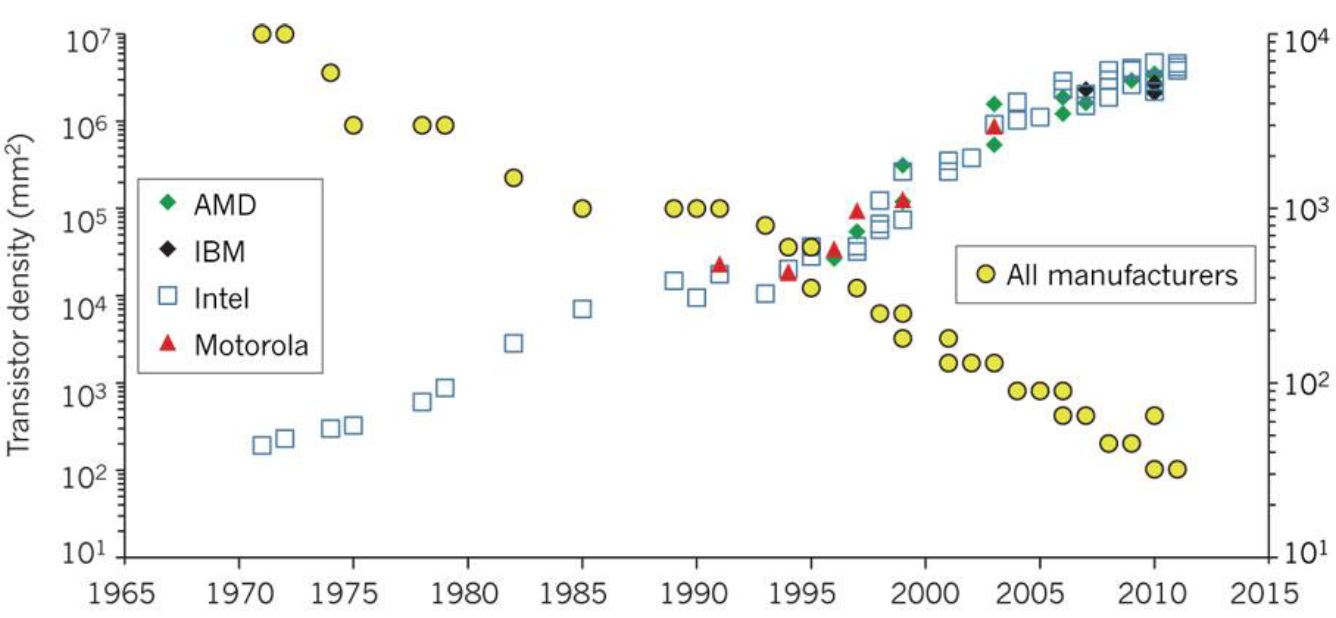
\includegraphics[width=\textwidth]{fig/moore1.png}
      \caption{Moore's Law. Source: \cite{quantum_computers}}
    \end{figure}
  \end{minipage}
  \begin{itemize}
    \item Moore's Law: The number of transistors on a microchip would double every two years, while the cost would be halved.
\end{itemize}
\end{frame}
\note{In 1965, Gordon Moore, the co-founder of Intel, predicted that the number of transistors on a microchip would double every two years, while the cost would be halved(halfed). 

This prediction has been proven(prove) to be true for the past 50 years. 

The figure shows the growth of the number of transistors from 1965 to 2015, shown in blue. 
The feature size which describes the size of the transistor, shown in yellow gets smaller and smaller.

}


\begin{frame}[fragile]{The End of Moore's Law \& Future of Computers}
  \begin{figure}
    \centering
    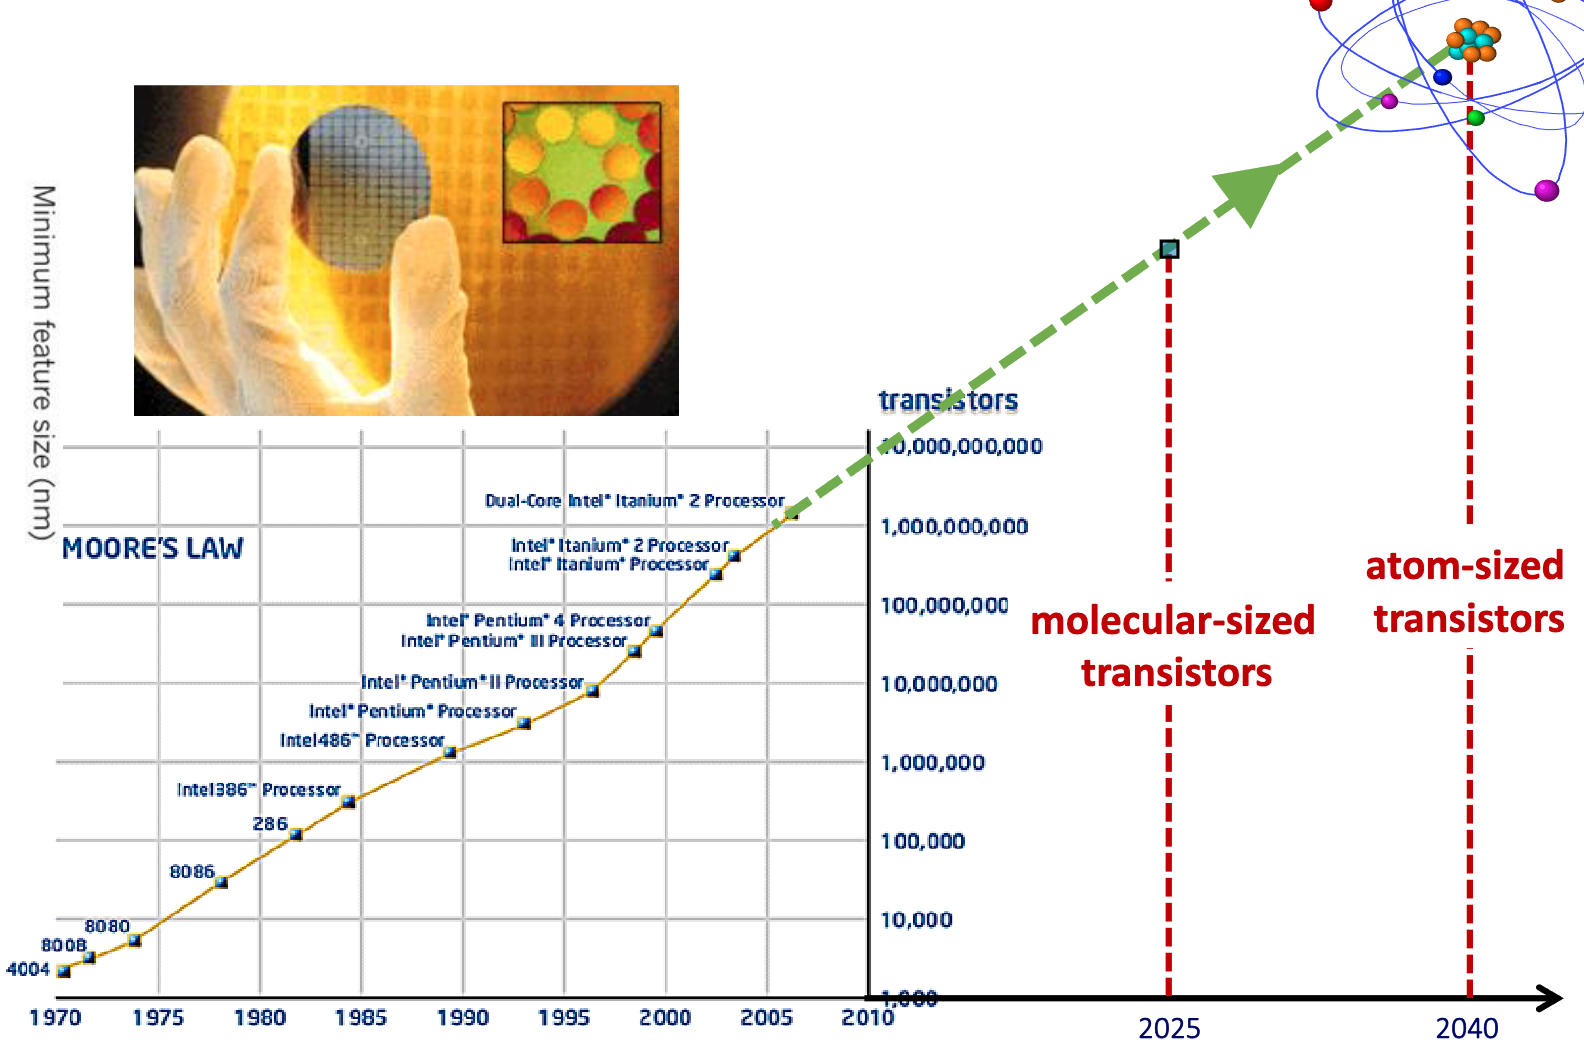
\includegraphics[width=0.8\textwidth]{fig/moore2.png}
  \end{figure}
  \begin{itemize}
    \item The feature size of the transistor is approaching the atomic scale.
    \item Quantum effects become significant.
    \item The development of new technologies is required.
  \end{itemize}
\end{frame}
\note{
  As the feature size of transistor approaches the atomic(a-tuo-mic) scale, Moore's law is facing challenges. 

In the atomic scale, the quantum effects become significant, and classical physics(phy-sic-s) is no longer valid.

This makes it impossible to continue the growth of the number of transistors on a microchip.

To continue the growth of computing power, the development of new technologies is required.

%Traditional silicon(ci-li-ken)-based computers are reaching their physical limits, and the development of new technologies is required to continue the growth of computing power. 

%Quantum computing is one of the most promising technologies that can potentially solve problems that are intractable(intra-ct-ble) for classical computers.
}


\begin{frame}[fragile]{Quantum Computers VS Classical Computers}
\begin{figure}
  \centering
  \begin{subfigure}[b]{0.2\textwidth}
    \includegraphics[width=\textwidth]{fig/google1.png}
  \end{subfigure}
  \hfill
  \begin{subfigure}[b]{0.3\textwidth}
    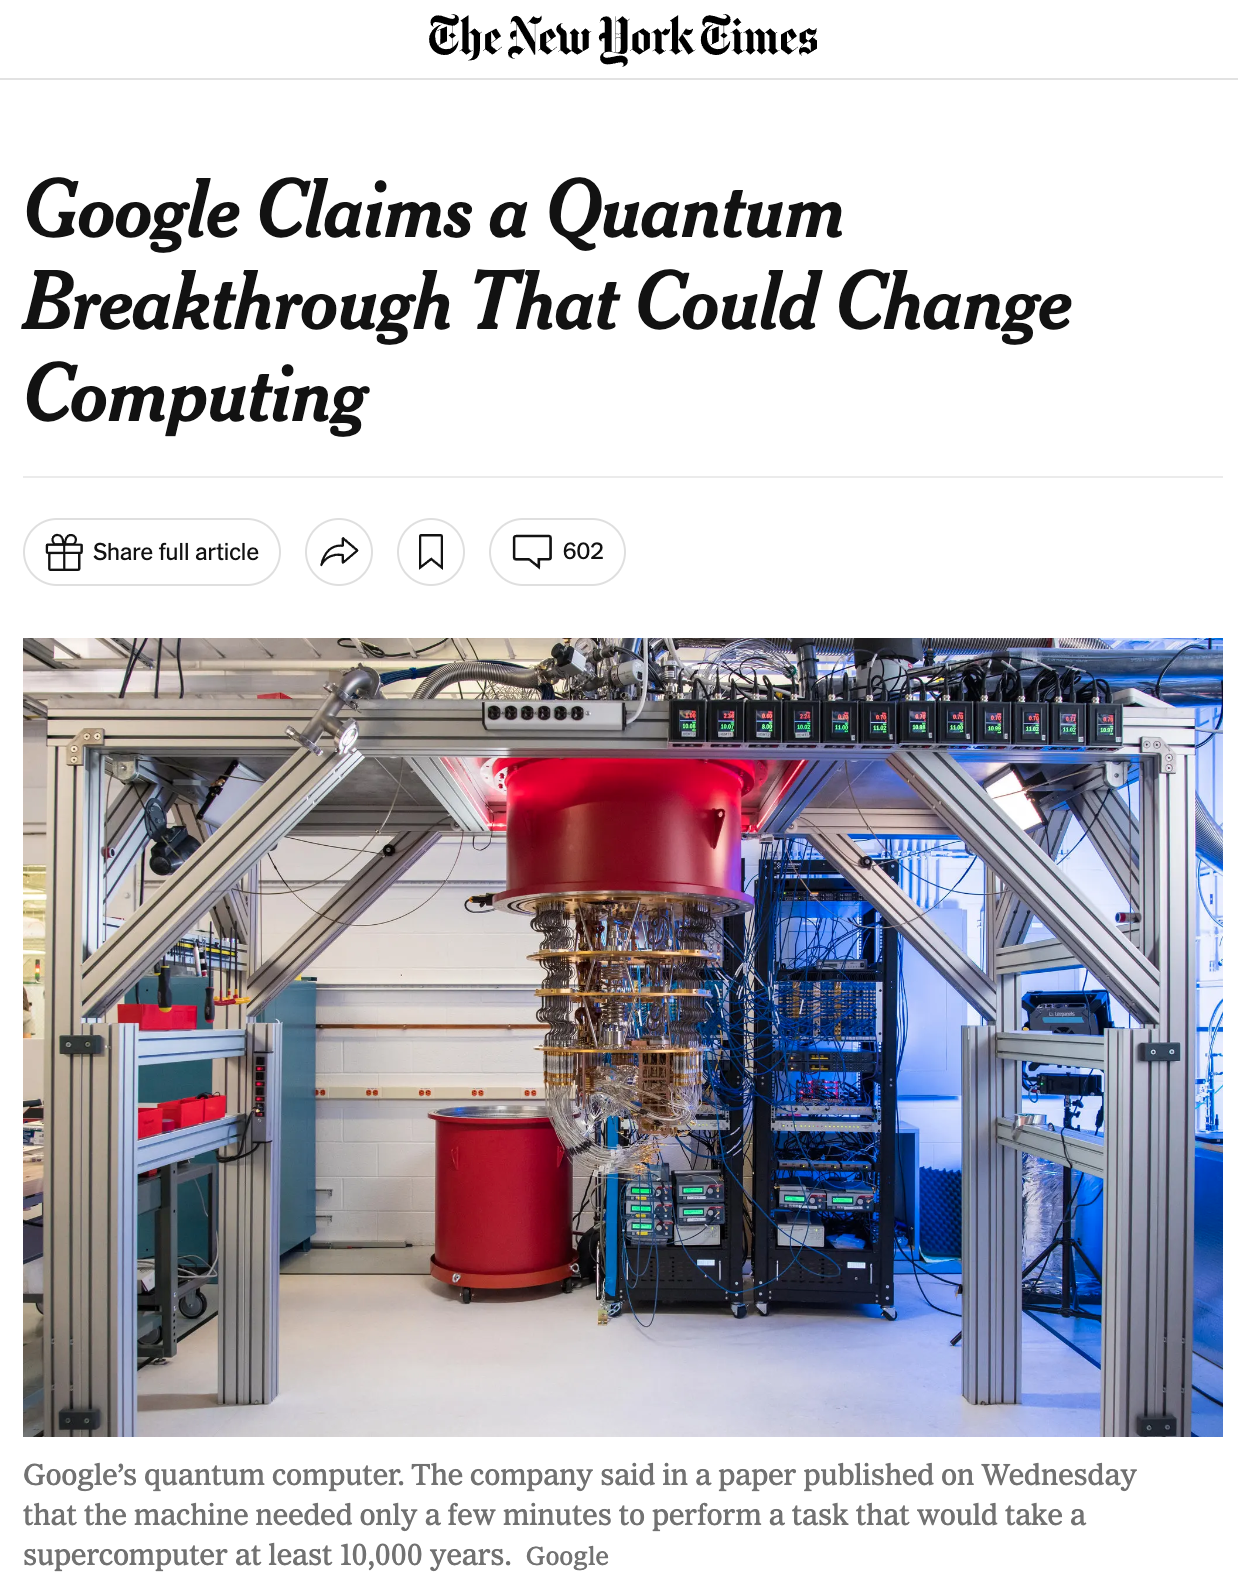
\includegraphics[width=\textwidth]{fig/newyorktimes.png}
  \end{subfigure}
  \hfill
  \begin{subfigure}[b]{0.4\textwidth}
    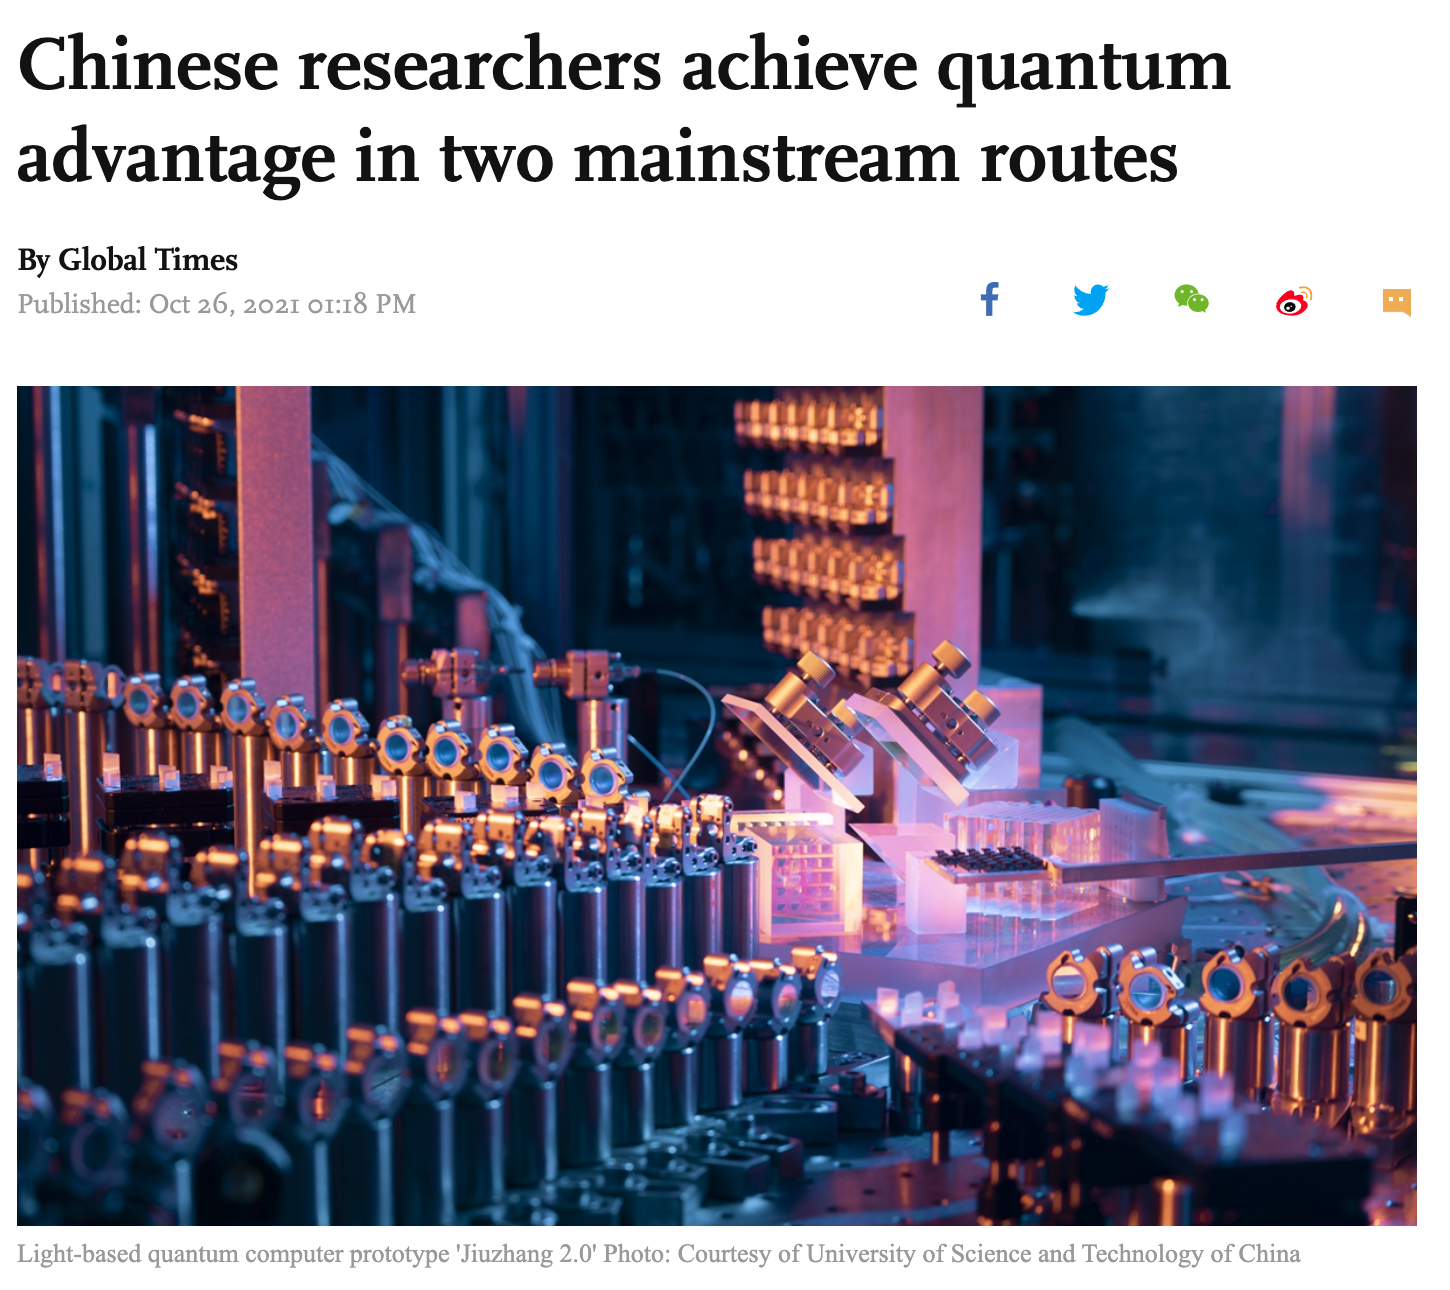
\includegraphics[width=\textwidth]{fig/chinatimes.png}
  \end{subfigure}
\end{figure}
\begin{itemize}
  \item Are quantum computers truly superior to classical computers?
  \begin{itemize}
  \item Quantum Advantage VS Classical Simulation.
  \end{itemize}
\end{itemize}
\end{frame}
\note{Recently, quantum computing has attracted(attract-ed) a lot of attention from both academia and industry(in-de-stry).

These are some reports about quantum computing from New york Times and Global Times.

Compared to classical computers, quantum computers are based on the principles of quantum mechanics(mi-can-ni-kes), such as superposition and entanglement. 


These properties bring a new look to computation. %and have the potential to solve problems that are intractable(intra-ct-ble) for classical computers.

The key question we’ll address is: if quantum computers are really better than classical computers?

There are two sides to this debate(\textipa{di'beit}).

One is the quantum advantage.
This term describes the quantum computers have the ability to complete computation task which are beyond the reach of classical computers.

For example, Google claimed(\textipa{kleimd}) their Sycamore quantum computer can perform a computation task in 200 seconds that would take the fastest supercomputer ten thousands years.

The other side is the classical simulation.
Some people argue that by find the weakness of the quantum computer, the classical computer can simulate the quantum computer efficiently.
For specific computation task, if efficient classical simulation can be achieved, the claims(\textipa{kleɪmz}) of quantum advantage in this task would be broken.

%Or using optimized algorithms and resources, the classical computer can still handle some tasks that quantum computers can do.




%Classical simulation techniques have advanced rapidly, narrowing the gap and challenging quantum supremacy claims. Some researchers argue that classical computers might still handle these tasks, albeit with optimized algorithms and resources.
%For example, last month Google announced their new quantum chip "Willow"(wei-low), which can solve a problem in 5 minutes that would take the world's fastest(fas-test) supercomputer in 10 septillion(sep-ti-lian) years.

%But what is quantum computing? And how does it work? Let's review the history of quantum computing.
}

\begin{frame}[fragile]
  Simulation of quantum circuits based on Pauli path integral:
  \begin{itemize}
    \item \textbf{Part 1:} A classical simulation method for a broad class of quantum algorithms, 
    with \textcolor{blue}{polynomial} cost in the presence of noise.
    \item \textbf{Part 2:} A classical simulation method for near Clifford quantum circuits,
    with \textcolor{blue}{polynomial} cost in noiseless case.
    \begin{itemize}
      \item \textbf{Variational Quantum Algorithms (VQAs).}
      \item Circuits with Clifford gates and Pauli rotation gates\footnote{Pauli rotation gates: $U(\theta)=e^{-i\frac{\theta}{2}P}$, where $P\in\{I,X,Y,Z\}^{\otimes n}$} under Pauli noise.
    \end{itemize}
  \end{itemize}
\end{frame}
\note{
  Today I will introduce our recont work on this topic.
  We propose a classical simulation method which can simulate a broad class of quantum algorithms with polynomial scale cost.

  The quantum algorithms we consider is the variational quantum algorithms, whose circuits are composed of Clifford gates and Pauli rotation gates in the presence of Pauli noise.
  I will introduce it later.
}


\begin{frame}[fragile]{Historical Background}
  \begin{figure}
    \centering
    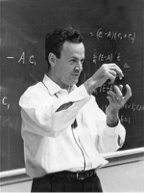
\includegraphics[width=0.2\textwidth]{fig/feynman.png}
  \end{figure}
  \begin{itemize}%~\footcite{feynman2018simulating}
    \item In the 1980s, Yuri Manin and Richard Feynman proposed the idea of quantum computing.
    \item \textbf{Motivation:} When classical computers simulate quantum systems, the cost grows \textcolor{red}{exponentially} with the number of particles. 
    \item \textbf{Solution:} Build a computer based on quantum mechanics.
    %\begin{itemize}
    %    \item Quantum simulation: simulate quantum systems efficiently.
    %\end{itemize}
  \end{itemize}
  \textbf{Key Questions:}
  \begin{itemize}
    \item How do we develop \textbf{useful quantum algorithms}?
    \item How do we handle \textbf{quantum noise}?
  \end{itemize}
\end{frame}
\note{
  In the 1980s, Yuri Manin(ma-ni) and Richard Feynman independently proposed the idea of quantum computing.

  The motivation is that when classical computers simulate quantum systems, the cost grows exponentially with the number of particles.

  A possible solution is to build a computer based on quantum mechanics.

  But there are two key questions to be addressed.
  First, at that time, there is no useful quantum algorithms. And people are not sure whether quantum algorithms are really better than classical algorithms.

  Second, the quantum noises are unavoidable(un-avoid-able) in quantum systems, which will destroy the quantum information.
  How to protect the quantum information from noise is a key issue in quantum computing.
  

%Feynman pointed out that when classical computers simulate quantum systems, as the number of particles increases, the time required for calculation will increase exponentially. %which is completely incompetent(in-com-pe-tent). 

The solution is to build a computer based on quantum mechanics. 

%This motivation is called quantum simulation, which aims to simulate quantum systems efficiently. 

%And it remains one of the core purposes of building quantum computers today.
}


\begin{frame}[fragile]{Shor's Algorithms}
  Useful quantum algorithms:
  \begin{itemize}
    \item In 1994~\footfullcite{shor1994algorithms}, Peter Shor proposed a quantum algorithm that can factorize large numbers in \textcolor{red}{polynomial time}.
    %\item Large numbers factorization: Knowing big number $N$, which is the product of two prime numbers $p$ and $q$. What are $p$ and $q$?
    \begin{itemize}
      \item \textbf{Classical Algorithms:} Best known algorithm require \textcolor{red}{sub-exponential} time.
      %\item The intractability of the factorization problem is the cornerstone of modern encryption.
    \end{itemize}

    \vspace{1em}
    \begin{figure}
      \centering
      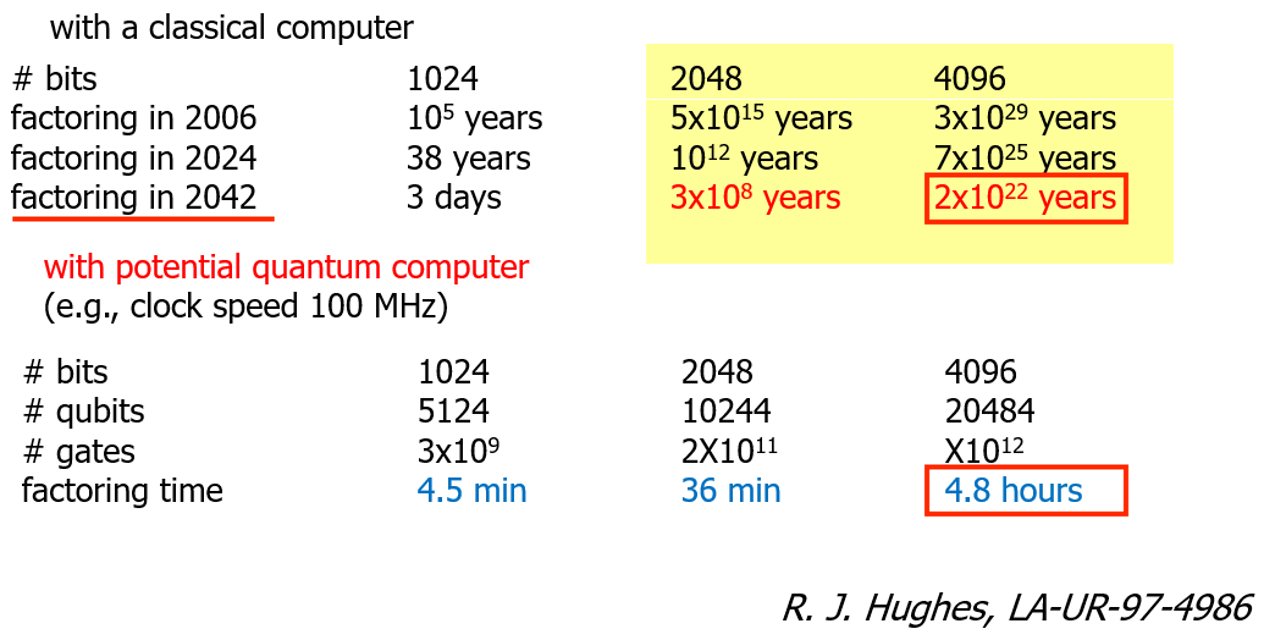
\includegraphics[width=0.6\textwidth]{fig/shor.png}
    \end{figure}
    %\item In 1996~\footcite{grover1996fast}, Lov Grover proposed a quantum algorithm that can search an unsorted database in \textcolor{red}{quadratic time}, while the best classical algorithm is \textcolor{red}{linear}.
  \end{itemize}
\end{frame}
\note{
A breakthrough in quantum algorithms came in 1994.  
In 1994, Peter Shor proposed a quantum algorithm that can factorize(fact-rize) large numbers in polynomial time.

The factorization of large numbers is a classic problem.% in number theory(see-ri). 
Given a big number N, which is the product of two prime(pri-me) numbers p and q. The  question is what p and q are?

The best classical algorithm for factorization is sub-exponential(ex-po-nential) time.

The intractability(intra-ct-a-bile-ty) of the factorization problem is the cornerstone(cor-ner-stone) of modern encryption(en-cre-pu-tion), such as RSA.

%And the quantum algorithm poses(po-ses) a threat(si-rea-te) to the security of many commercial encryption systems.

Here is a comparison(com-par-re-sen) between the classical and quantum algorithms for factorization.

It is estimated that a 4K-length RSA key can be broken in 4 hours by shor's algorithm. While even for classical computers in 2042, it will take 10 to 22 years.}


\begin{frame}[fragile]{Quantum Error Correction}
  Protect quantum information from noise:
  \begin{itemize}
    \item Noise is inevitable in quantum systems.
    \item Peter Shor~\footfullcite{shor1995scheme} proposed to use error correction codes to protect quantum information from noise.
    %\begin{itemize}
      %\item Quantum error correction codes: encode quantum information in a larger Hilbert space.
      %\item Quantum error correction is difficult due to the properties of quantum mechanics.
      %\begin{itemize} 
      %\item No-cloning theorem
      %\item Collapse of the wave function
      
      %\dots
      %\end{itemize}
    %\end{itemize}
  \end{itemize}
\end{frame}
\note{%Depending on complexity theory, quantum computers are believed to be able to solve certain problems exponentially faster than classical computers.

After the proposal of Shor's algorithm, the actual construction of quantum computers becomes a hot topic. Academia, industry, and even governments have invested a lot of resources in this field.

However, the development of quantum computers is not as smooth as expected(ex-pec-ted). 

The quantum information is easily destroyed by the environment, leading to a process(pro-cess) called decoherence.

To protect quantum information from noise, Peter shor proposed to use error correction codes to encode quantum information in a larger Hilbert space.
Which is a promising way to protect quantum information.


However quantum error correction is difficult to perform. %due(du-to) to the properties of quantum mechanics, such as the no-cloning(clone-lin) theorem(see-rem) and the collapse(co-la-pse) of the wave function.
}

\begin{frame}[fragile]{Error Correction is Expensive}
 The implementation of quantum error correction is described in seven stages, described in 2013. %Each advancement requires mastery of the preceding stages, but each also represents a continuing task that must be perfected in parallel with the others. Superconducting qubits are the only solid-state implementation at the third stage, and they now aim at reaching the fourth stage (green arrow). In the domain of atomic physics and quantum optics, the third stage had been previously attained by trapped ions and Rydberg atoms. No implementation has yet reached the fourth stage, where a logical qubit can be stored, via error correction, for a time substantially longer than the decoherence time of its physical qubit components.
  \begin{figure}
    \begin{tikzpicture}
      \node[anchor=south west,inner sep=0] (image) at (0,0) {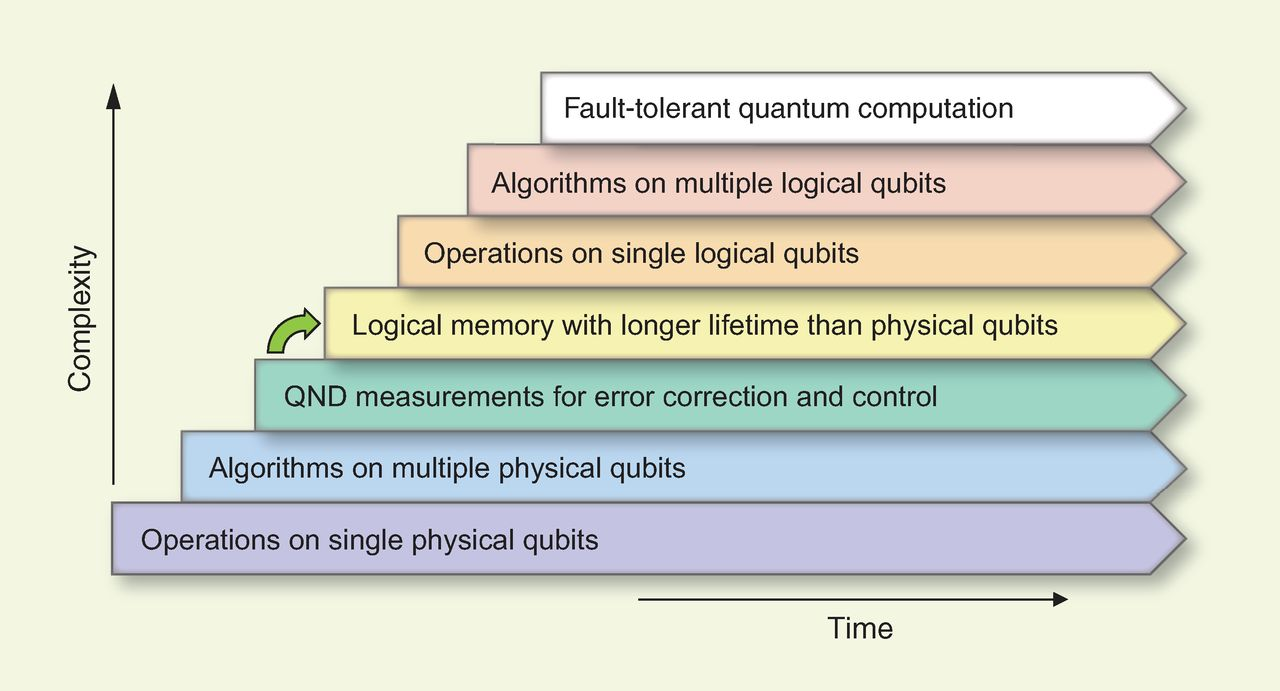
\includegraphics[width=0.9\textwidth]{fig/339_1169_f1.jpeg}};
      \begin{scope}[x={(image.south east)},y={(image.north west)}]
        \draw[red,thick,<-] (0.8,0.85)--(0.85,0.9) node[anchor=south west] {Factoring Algorithm};
      \end{scope}
    \end{tikzpicture}
    \footcite{devoret2013superconducting}
  \end{figure}
  \begin{itemize}
    \item After 10 years, \cite{ni2023beating}(USTC) and \cite{acharya2024quantum}(Google) reached the fourth stage.
  \end{itemize}
\vspace{0.5em}
\end{frame}
\note{The implementation of quantum error correction is described in seven stages, as shown in the figure. 

%Each advancement requires mastery of the preceding stages, but each also represents a continuing task that must be perfected in parallel with the others.

In 2013, we were at the third stage and tried to reach the fourth stage, as the green arrow shows.

The third stage describes the necessary operations for quantum error correction such as measurement and control can be performed.

The fourth stage is the logical qubit has a longer coherence time than the physical qubits.

In other words, it describes the error correction scheme(si-game) can bring positive effects in the real quantum devices.

Actually after 10 years, marked by USTC in last year, and Google Willow in last month, the quantum error correction reaches the fourth stage.

While the Shor's factorization algorithm is at the top stage.
}



\begin{frame}[fragile]{Noisy Intermediate-Scale Quantum (NISQ) Computers}
 %Fault-tolerant quantum computers are still far from reality. 
 Nowadays Quantum devices have entered the NISQ era, with the potential to achieve quantum advantages.
  \begin{itemize}
    \item \textbf{Qubit Count:} 50--1000 qubits
    \item \textbf{Gate Fidelity:} 99.9\%--99.999\% (still \textcolor{red}{noisy})
    %\item Limited connectivity: \textcolor{red}{nearest-neighbor} (superconducting qubits)
  \end{itemize}
  \begin{figure}
    \centering
    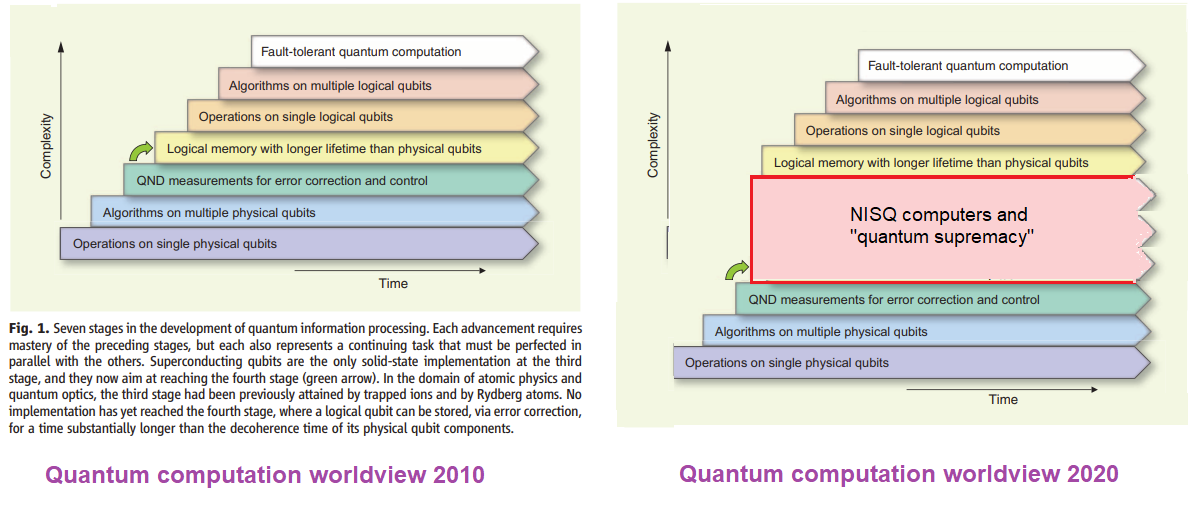
\includegraphics[width=0.9\textwidth]{fig/2010-2020d.png}\footcite{nisq}
    %\caption{Source: \footcite{nisq}}
  \end{figure}
  \begin{itemize}
    \item Around 2020, exploring the potential of NISQ devices to achieve quantum advantages.
  \end{itemize}
  \vspace{0.25em}
\end{frame}
\note{%Fault-tolerant(fou-te-to-le-rant) quantum computers can perform quantum computation reliably(relai-a-bo-ly). But the fault-tolerant quantum computers are still far from reality(re-a-lity).

Nowadays, quantum devices have entered the NISQ era, which stands for the Noisy Intermediate-Scale Quantum era. It is characterized(\textipa{ˈkærəktəˌraizd}) by the following features:

It has hundreds qubits, typically between 50 to 1000.

The gates are imperfect, with probabilities to introduce errors. 

% And the connectivity of the gates is limited. Not all qubits can interact with each other directly.

Because the error correction is still far from now.

As the right figure shows. 

Around 2020, a new direction is emerging(\textipa{ɪˈmɜːdʒɪŋ}) to explore the potential of NISQ devices to achieve quantum advantages. 
}


\section{Variational Quantum Algorithms}
\note{
  The Variational Quantum Algorithm are the most popular quantum algorithms in the NISQ era.
}

\begin{frame}[fragile]{Variational Quantum Algorithms}
 Variational quantum algorithms (VQAs) are a class of quantum algorithms designed for NISQ devices. %, and are widely recognized as a potential pathway to achieve practical quantum advantages.
  \begin{figure}
    \centering
    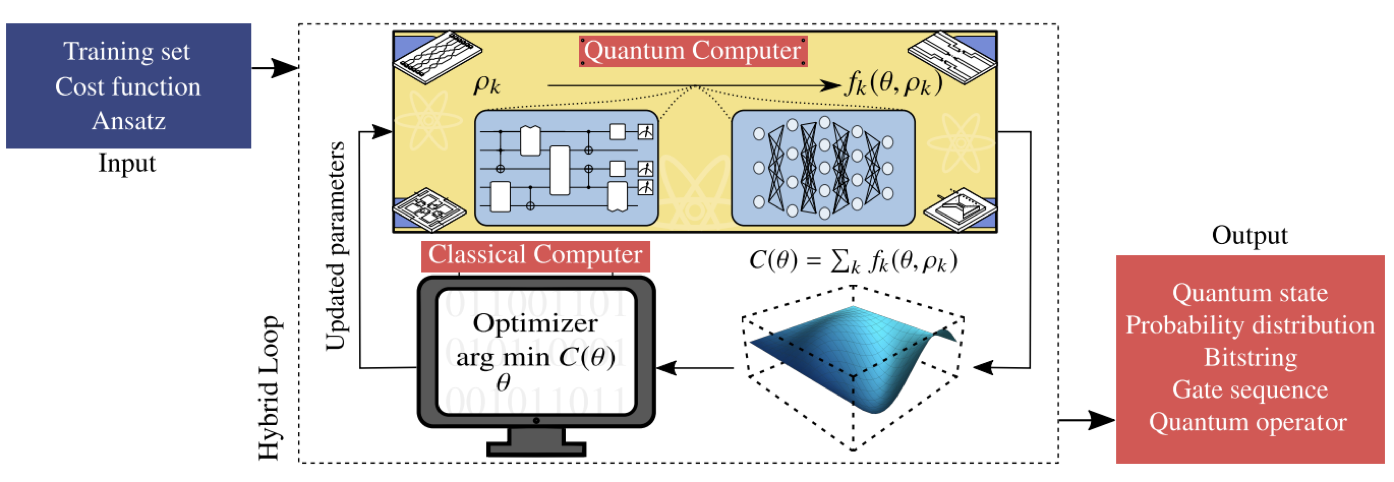
\includegraphics[width=0.7\textwidth]{fig/vqa.png}\footcite{Cerezo2021variational}
  \end{figure}
  
  

  \begin{itemize}
    \item \textbf{Parameterized Quantum Circuits}: Serve as the model, analogous to neural networks in deep learning.
    \item \textbf{Quantum Processor}: Executes the quantum circuits, acting as a co-processor.
    \item \textbf{Classical Optimizer}: Adjusts the circuit parameters to minimize the loss function, iteratively improving the solution.
  \end{itemize}
  \vspace{1em}
\end{frame}
\note{
 Variational quantum algorithms are a class of quantum algorithms designed for NISQ devices and have the potential to achieve practical quantum advantages without error correction.

 It combines quantum computer with classical computer.
 
 In some ways, Variational quantum algorithms can be viewed as a quantum version of Neural(\textipa{ˈnʊrəl}) Networks.

 The difference is using parameterized(per-ramite-rized:\textipa{pə'ræmitəraizd}) quantum circuits instead of artificial neural networks as learning models.


 The quantum computer is used as a co-processor to run the model and evaluate the loss function.
  
 Then, a classical computer is used to %iteratively(it-rea-tively) 
 adjust these parameters(per-ramiter-s) to minimize the loss function, and searching for the optimal solution.
  
 %It’s like searching for the best formula or strategy for solving a problem.
}


\begin{frame}[fragile]{Variational Quantum Algorithms}
 Many applications of variational quantum algorithms have been proposed, including:
  \begin{itemize}
    \item Hamiltonian simulation~\footcite{chen2020demonstration}
    \item Combinatorial optimization (QAOA)~\footcite{farhi2014quantum,moll2018quantum}
    \item Quantum chemistry (VQE)~\footcite{peruzzo2014variational, Kandala2017hardware,li2022toward}
    \item Quantum machine learning (QDNN, QGAN, QCNN)~\footcite{beer2020training,huang2021experimental,havlivcek2019supervised,mitarai2018quantum}
    \item Quantum circuit compilation~\footcite{khatri2019quantum}
    \item Quantum error correction~\footcite{johnson2017qvector,xu2021variational}
    \item ....
  \end{itemize}
  \vspace{1em}
\end{frame}
\note{
Many applications of variational quantum algorithms have been proposed, including 
Hamiltonian simulation, which is to use quantum computers to simulate the evolution(\textipa{/ˌevə'lu:ʃ(ə)n/}) of quantum systems.
 As well as solving combinatorial(com-bina-torial) optimization problems, quantum chemistry(\textipa{'kemistri}), and machine learning, and in return provides solutions in quantum computation fields.

 Like the quantum circuit compilation(com-pi-lation), quantum error correction, and so on.
}

\section{Simulating Noisy Variational Quantum Algorithms}
\begin{frame}[fragile]
  Whether the quantum advantage of variational quantum algorithms can be maintained in the presence of \textcolor{red}{noise}?

  \fullcite{shao2024simulating}
   \begin{itemize}
     \item \textbf{Simulation Method:} A method to simulate the noisy observable value of variational quantum algorithms without assumptions of locality, low entanglement entropy, or circuit depth.
     \item \textbf{Cost:} Prove that the simulation cost is \textcolor{red}{polynomial} scale when simulation error is bounded by a given threshold with high probability.
     %\item Provide a theoretical analysis of the quantum advantage in noisy variational quantum algorithms.
     %\item Develop a high-performance program to implement the simulation method and apply it to simulate IBM's 127-qubit experiment.
   \end{itemize}
 \end{frame}
 \note{
  Variational quantum algorithms are designed for NISQ devices, which are noisy. A question is whether the quantum advantage can be maintained in the presence of noise.

   To address this question, let me introduce our recent work.
 
  It is a joint work with my mate Wei Fuchuan, Professor Cheng Song and my supervisor Professor Liu Zhengwei.
 
  In this work, we propose a method to simulate the noisy observable value of variational quantum algorithms without assumptions(\textipa{ə'sʌmpʃən}) of locality, low entanglement entropy, or circuit depth.
 
  And we rigorously(ri-go-rous-ly;\textipa{'rigərəsli}) prove that the simulation cost is polynomial scale when the simulation error is bounded by a given threshold with high probability.

  This work indicates that, considering the current(ca-rent) experimental capabilities(ca-pu-bilities), most variational quantum algorithms can be classically simulated. 

  
  %We also develop a high-performance program to implement the simulation method and apply(\textipa{ə'plai}) it to simulate IBM's 127-qubit experiment.
}

\begin{frame}[fragile]{IBM's 127-qubit expriments}
 In 2023, IBM~\footfullcite{kim2023evidence} demonstrated a 2D Ising model simulation task on a 127-qubit quantum computer and claimed it as evidence of the utility of quantum computing.
  \begin{figure}
    \centering
    \begin{subfigure}[t]{0.3\textwidth}
      \vtop{\null\hbox{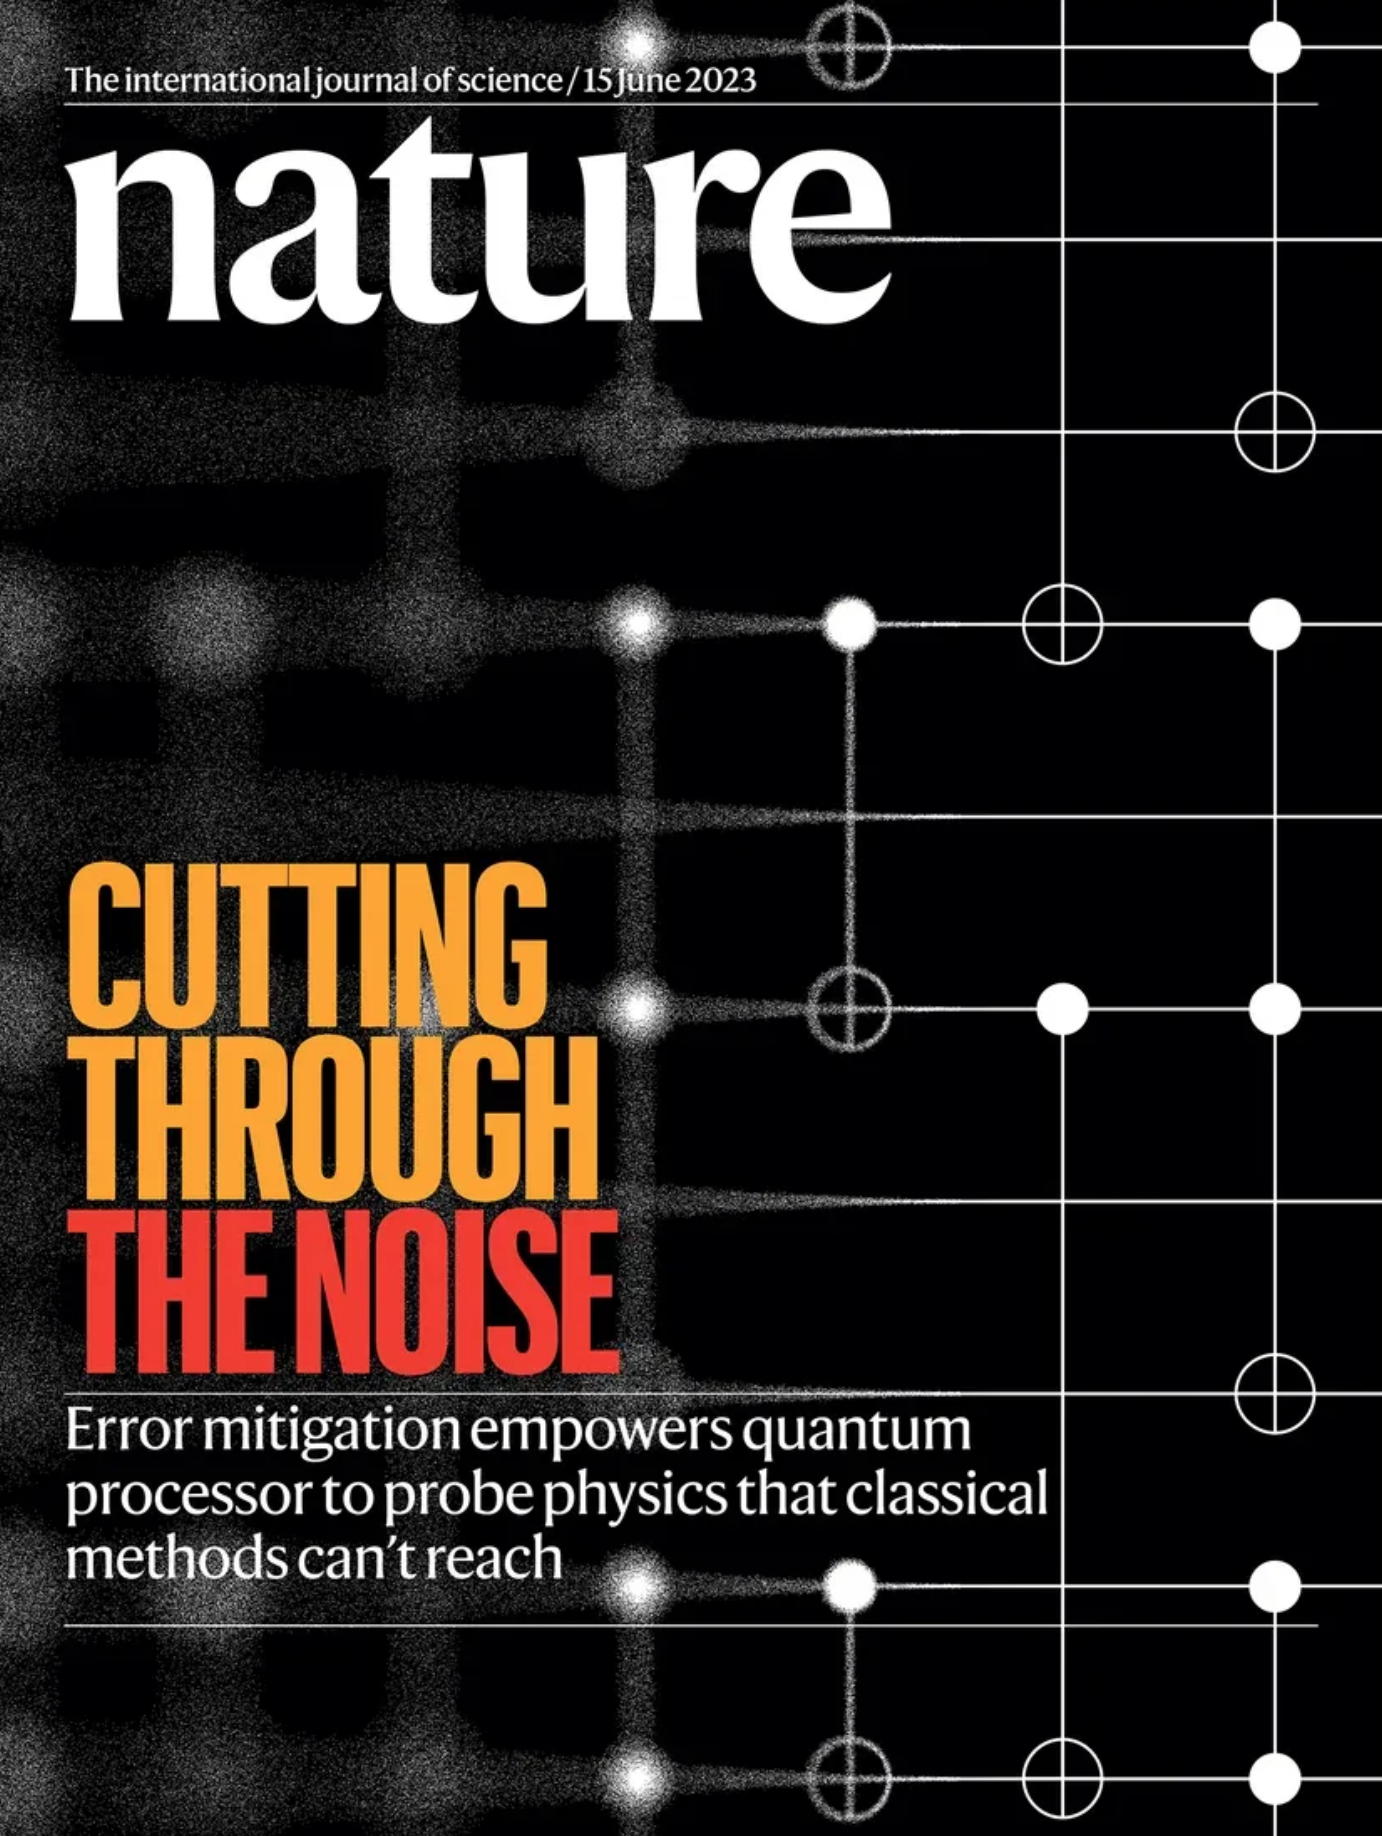
\includegraphics[width=\textwidth]{fig/ibm1.png}}}
    \end{subfigure}
    \hfill
    \begin{subfigure}[t]{0.65\textwidth}
      \vtop{\null\hbox{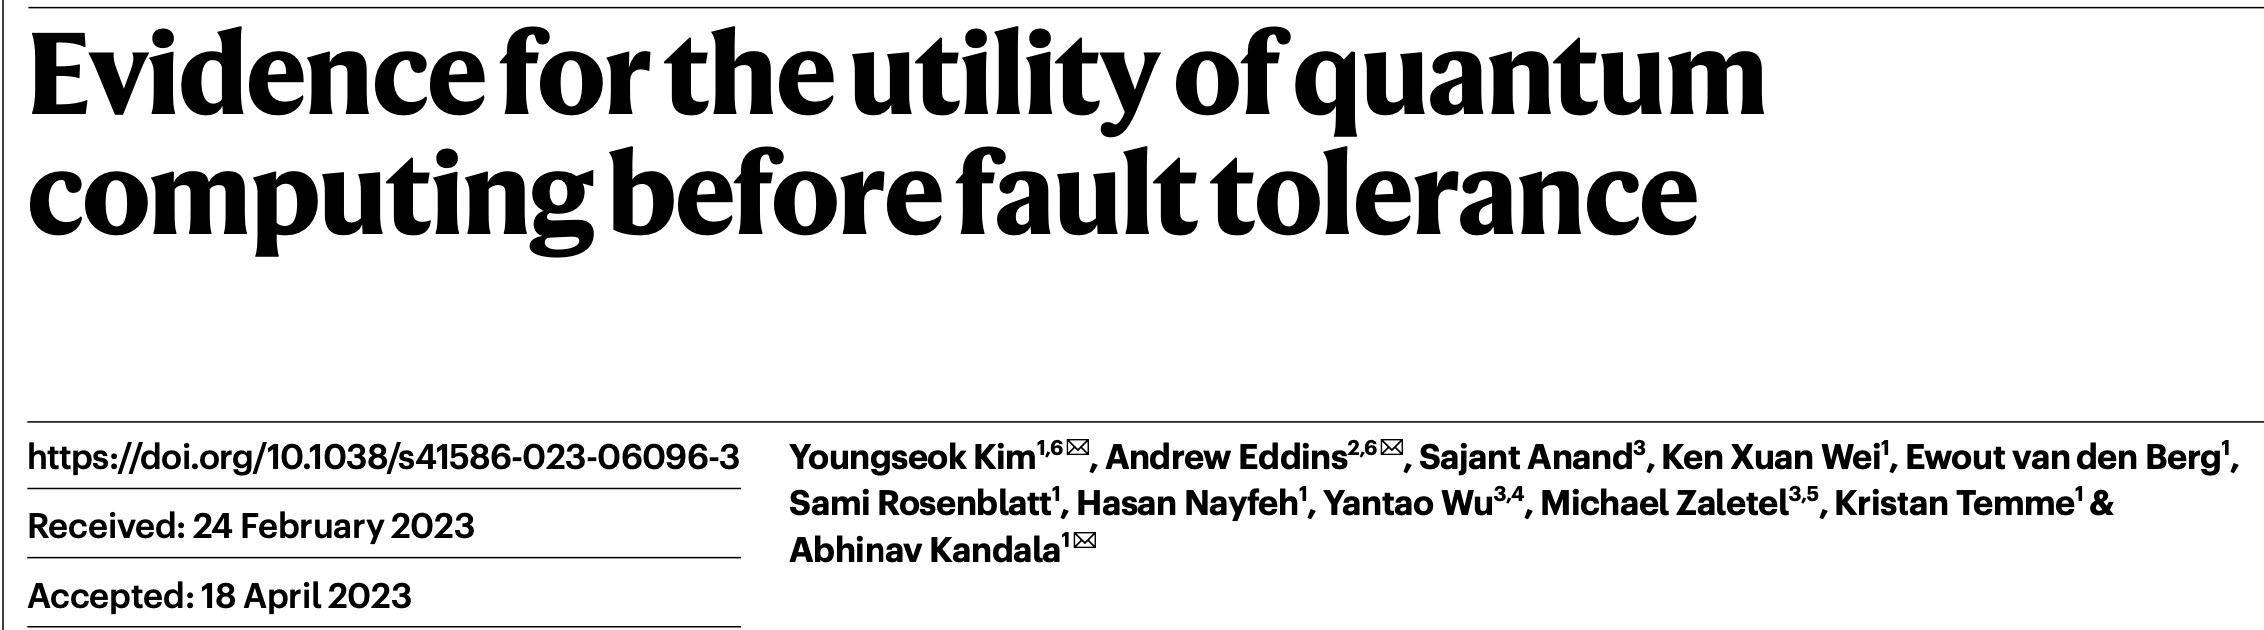
\includegraphics[width=\textwidth]{fig/ibm2.png}}}
      %\vtop{\null\hbox{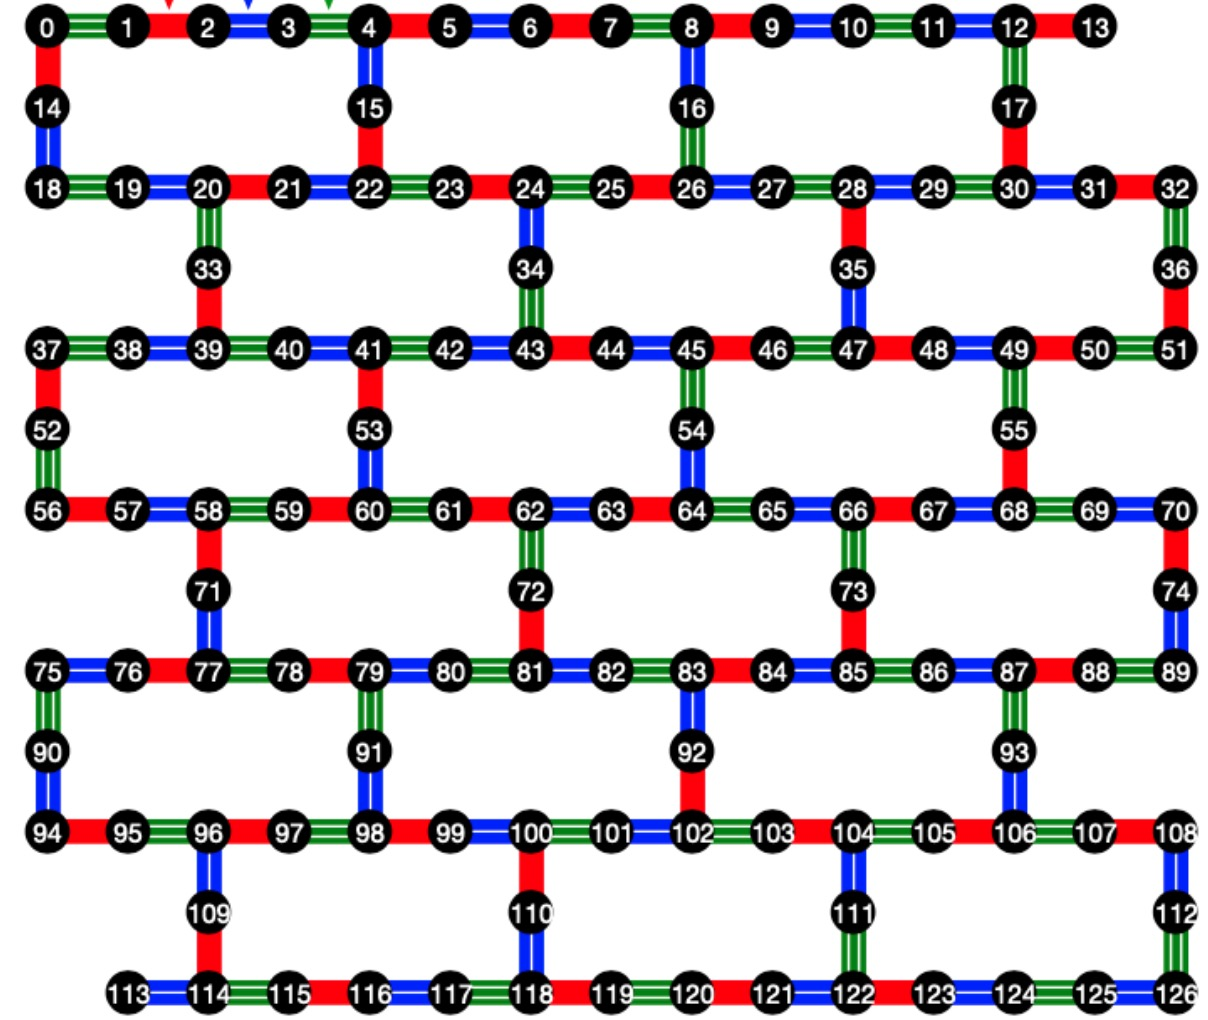
\includegraphics[width=0.6\textwidth]{fig/ibm3.jpg}}}
    \end{subfigure}
  \end{figure}
\end{frame}
\note{
  After we find this method, we need to find a good example to test it.

  At that time, we noticed a paper on the cover of Nature.

In this paper, IBM demonstrated(demo-strated) a 2D Ising model simulation task on 127-qubit quantum computer. 
  
%Simulating 2D Ising model is a challenging task for classical computers.
The exact simulation of 2D lattice quantum devices is a challenging task for classical computers.

And they claimed that this experiment is the evidence of the utility(u-ti-lety) of quantum computing.

This experiment is a typical example of variational quantum algorithm.
And we apply our simulation method to simulate this experiment.
   
  %The Ising model is fundamental in statistical(\textipa{/stə'tistik(ə)l/}) mechanics, and it is widely used in many fields.
 
  %
 
  %IBM claimed that this experiment is the evidence of utility of quantum computing.
 }

 \begin{frame}[fragile]
  \begin{figure}
    \centering
    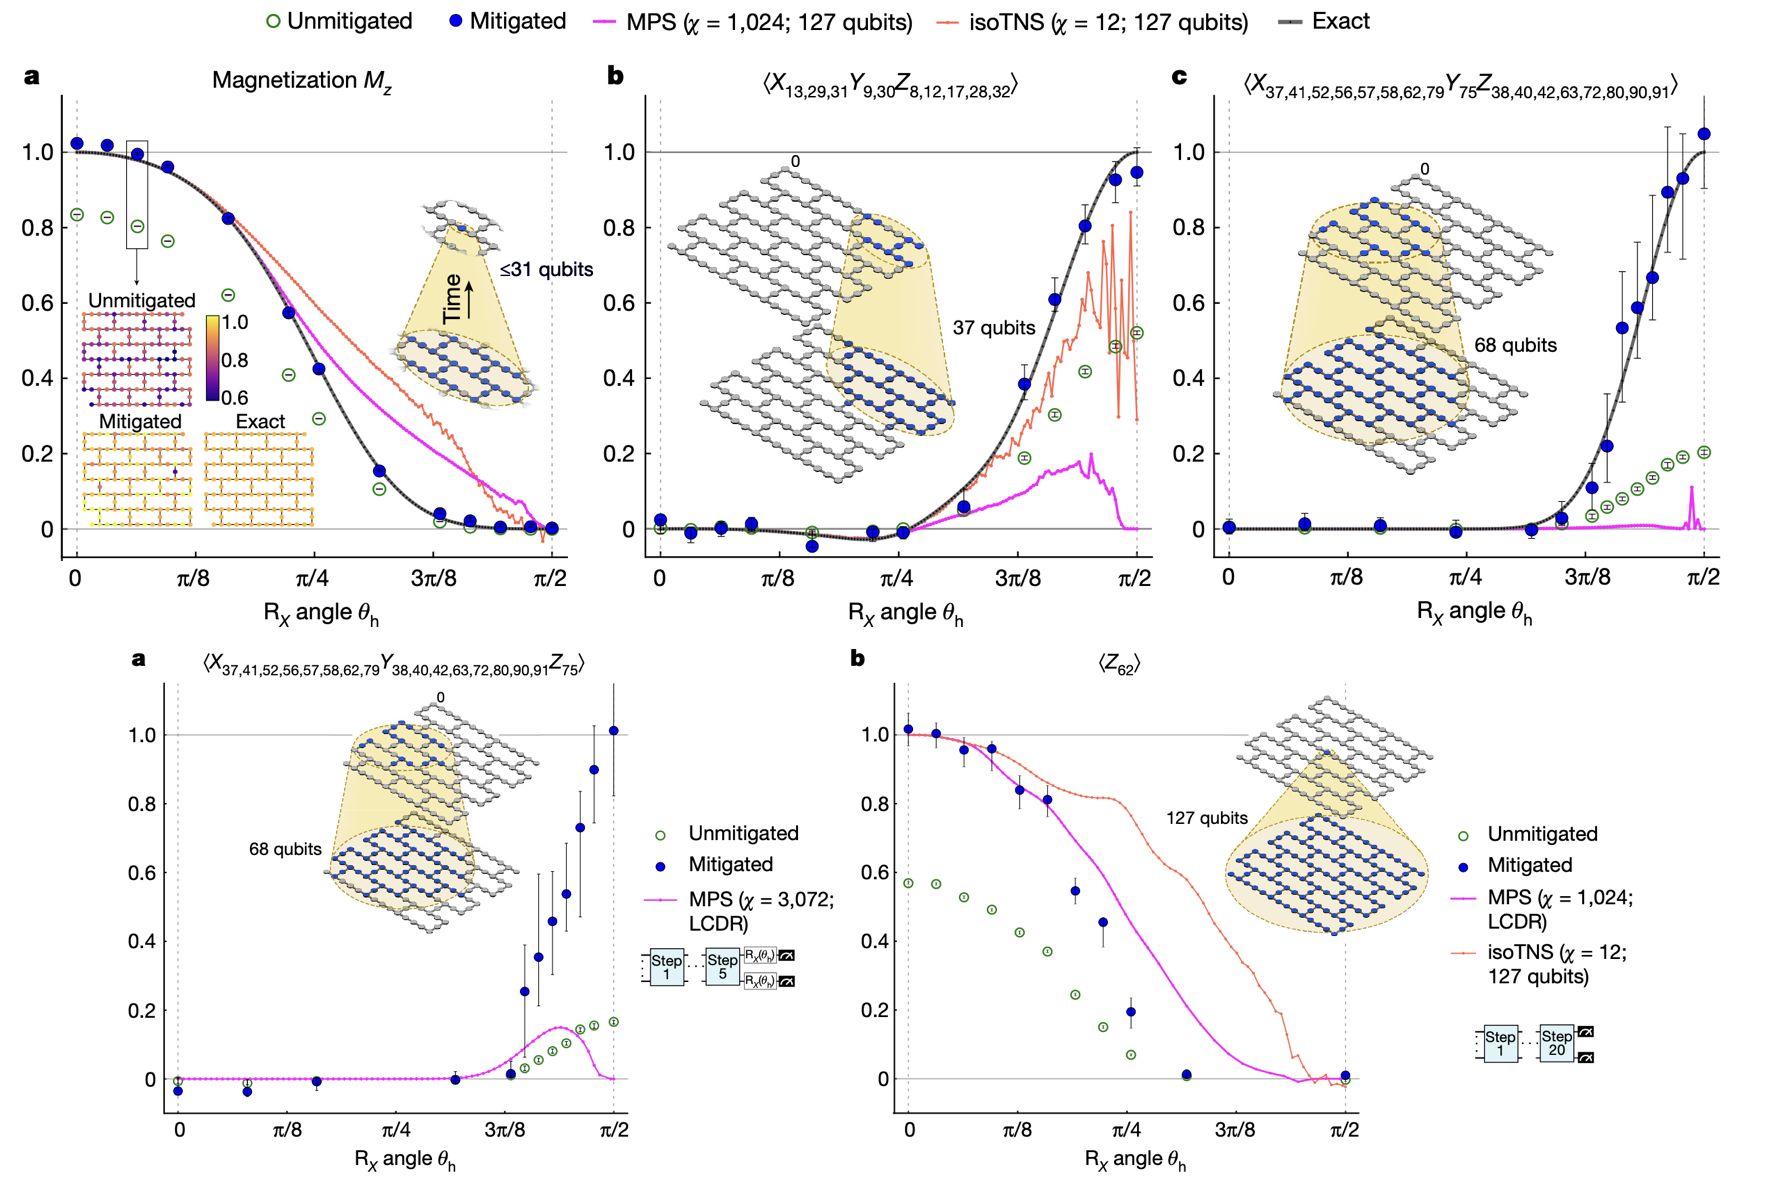
\includegraphics[width=0.95\textwidth]{fig/ibm4.png}
  \end{figure}
   \vspace{-1em}
   \footnote{Experimental data:\\
    \textcolor{blue}{Blue points} Mitigated results: Use Zero noise extrapolation (ZNE) to estimate noiseless results from noisy experimental data.\\
  \textcolor{green}{Green points} Unmitigated results: Noisy raw experimental data.\\}
\end{frame}
 \note{\scriptsize

 Let's look at at the footnote first.
 The experimental data from IBM contains two parts.
  The mitigated results which is the noise mitigated results obtained by using the zero noise extrapolation(extra-polation) method, is drawn in blue points.
  
The ZNE is a error mitigation method that estimates noiseless results from the noisy experimental data.

And the second part are the unmitigated results which are the noisy raw experimental data obtained directly from the quantum computer, is drawn in green points.


Let's see the first figure. 
In the first figure, the observable operator is weight one and the circuit is not deep, by light cone method, the involved qubits number is therety-one, thus the ideal exact results can be obtained.

  
 And the ideal exact results are drawn in the black line.

 
  You can see that compared to the unmitigated results, the quantum computer's mitigated results labeled by blue points are consistent(con-sis-tent) with the black line.

  This means that the quantum computer can provide accurate results for this task.

  While for some classical tensor network methods such as 1D matrix product state and 2D isometric tensor network state, they are labeled as red and purple lines, which are far from the black line.

  The situation is similar in the top three figures.

  %In the bottom subfigures, where no ideal results are available, the pattern observed in the top figures suggests that the quantum computer's mitigated results remain reliable, whereas the tensor network methods produce incorrect results.



  For the bottom(\textipa{'bɒtəm}) figures, because there are too many qubits involved, there is no ideal result as a reference.
 
  The quantum computer and classical methods provide different results. But based on the previous(\textipa{ˈpri:viəs}) figures, IBM claimed the results from quantum computer are relatively reliable.
  
  
  %while these results obtained by the tensor network methods can be considered incorrect.


 %This experiment shows that the quantum computer can provide correct results for which the classical approximation fails.
}



 \begin{frame}[fragile]%{Numerical Simulation for IBM's 127-qubit expriments}
  \vspace{-1.5em}
    \begin{figure}
      \centering
    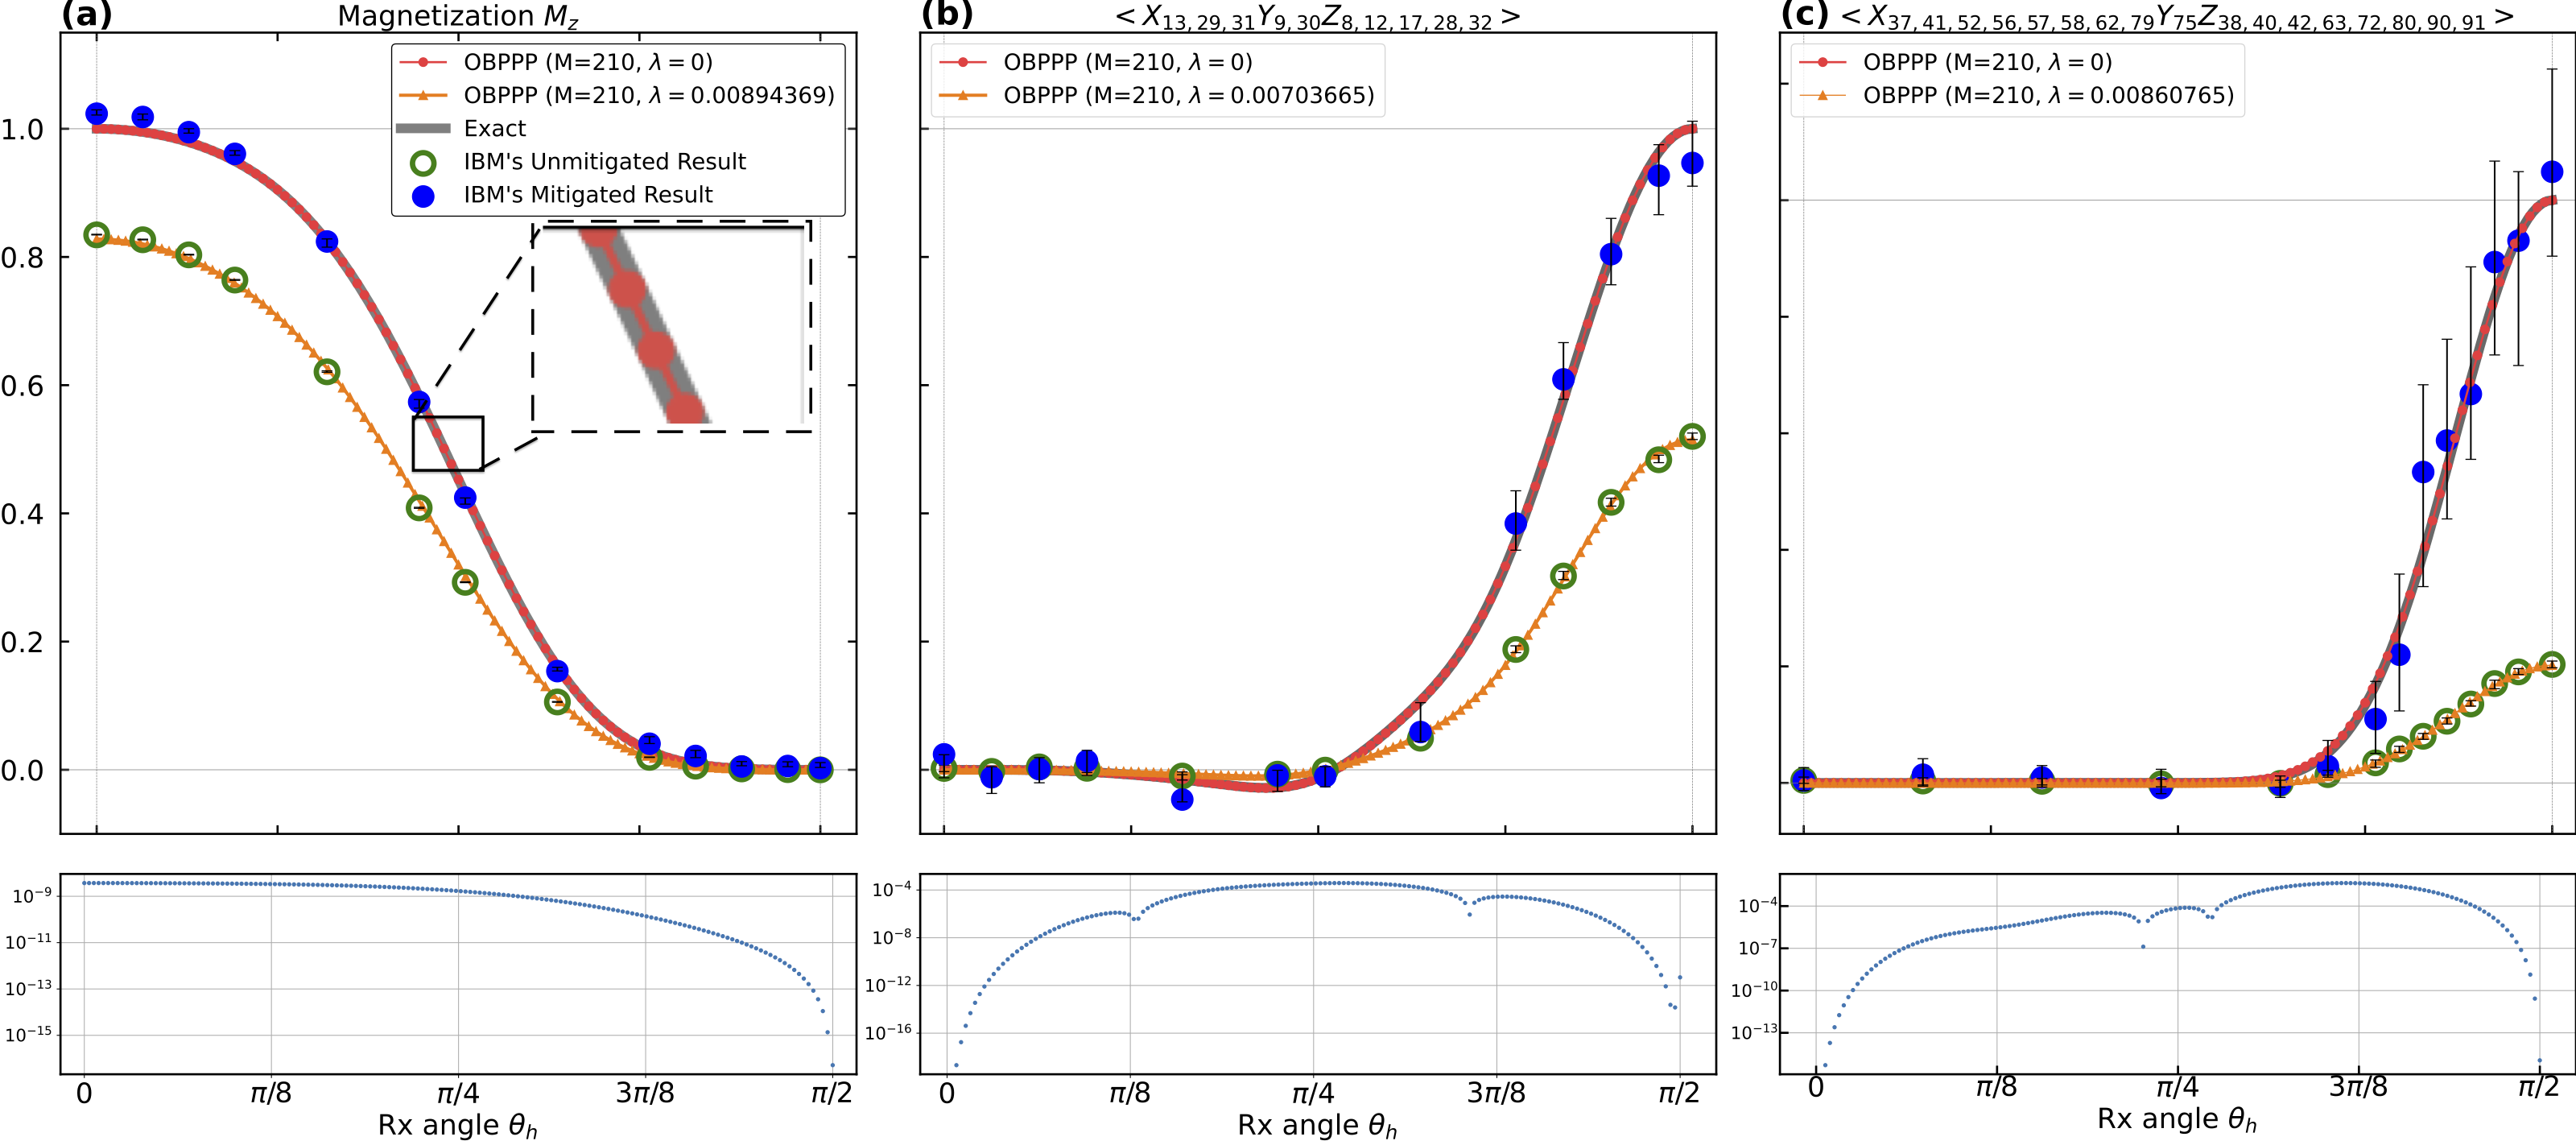
\includegraphics[width=1.05\textwidth]{fig/simibm1_zoom.png}
    \end{figure}
  \vspace{-1.5em}
  \textbf{Our Simulation results:}
  \vspace{-1em}
  \begin{itemize}
    \item \textcolor{red}{Red}(noiseless):Faster and more accurate than the Quantum computer.
    \item Outputs are \textbf{analytical expressions}, with the entire curve obtained in a \textbf{single run}.
    \item \textcolor{orange}{Orange}(noisy):Use unmitigated results to fit the noise rate, which is consistent with the noise rate reported by IBM. \small{(0.007-0.009)}
  \end{itemize}
  \vspace{-1em}
  \footnote{
    \textcolor{blue}{Blue points} Mitigated results.\\
  \textcolor{green}{Green points} Unmitigated results: Noisy raw experimental data.\\
  Runtime: Classical 13s, 146s, 29s vs Quantum 5 minutes(without post-processing).}
 %Noise is characterized by $p_x=p_y=p_z=\sfrac{\lambda}{4}$. Optimize $\lambda$ to fit the raw experimental data, getting the best fit $\lambda$ ranges from 0.007 to 0.009, which is consistent with the error rate reported by IBM.
\end{frame}
\note{\scriptsize

 Here are our simulation results for the top three figures in IBM's experiment.
 
 Our simulation results also contains two parts.

 First let me introduce the noiseless results.

Let's see the first figure.

 The noiseless simulation results are drawn in the red line, and the exact reference results are drawn in a black which is completely covered by the red line. As the zoom figure shows.

 Among the three figures, our simulation results are more accurate(a-curate:\textipa{ˈækjərət}) than the quantum computer.

And as the footnote shows, the running time for our classical simulation is only at most one hundred and fifty seconds, while the quantum computer would take 5 minutes even don't consider the classical post-processing time.

If considering the post-processing, the quantum computer would take many hours.

So our simulation are faster and more accurate than the quantum computer.

 By the way, the simulation outputs are not just values, but analytical(ana-ly-tical) expressions(\textipa{ik'spreʃ(ə)nz}) respect to the noise rate and rotation angles.

 The rotation angles are the x-axis(\textipa{'æksis}) in these figures.

So we can get the analytical expressions in a single run, and then bring in different rotation angles to get the entire(en-trie累) curve.

 And this makes it possible to add depolarizing(de-polar-rizing) noise to the simulation, and optimize the noise rate to fit the unmitigated results.

 %The raw experimental data is the original noisy expectation value of the quantum circuits without subsequent noise mitigation procedures.

 As the orange line shows, by optimizing the noise rate, our noisy simulation results are consistent with the quantum computer's raw experimental data.

 The optimized noise rate ranges from 0.007 to 0.009, which is consistent with the error rate reported by IBM.
}

\begin{frame}[fragile]{Properties}
  Key properties of our simulation method:
  \begin{itemize}
    \item \textbf{Analytical Outputs:}
    The simulation provides analytical expressions as functions of both the \textcolor{blue}{rotation angles} and the \textcolor{red}{noise rate}.
    \begin{enumerate}
    \item \textbf{Efficiency:}
    The entire curve can be computed in a single run.
    Bring in different \textcolor{blue}{rotation angles} to get points on the curve.
    \item \textbf{Noise Mitigated and Unmitigated Results:}
    \begin{itemize}
      %\item Setting the noise rate to zero to mitigate noise effects, providing an estimate of the \textcolor{red}{noiseless} results.
      \item By setting the noise rate to zero, the noise effects are mitigated, providing an estimate of the \textcolor{red}{noiseless} results.
      %\item Optimize the noise rate to fit the noisy unmitigated results, simulating the \textcolor{red}{noisy} raw experimental data.
      \item The noise rate can be optimized to fit the noisy unmitigated results, simulating the \textcolor{red}{noisy} raw experimental data.
    \end{itemize}
    %Setting the \textcolor{red}{noise rate} to zero to mitigate noise effects, providing an estimate of the noiseless results.
    %Optimize the \textcolor{red}{noise rate} to fit the noisy unmitigated results, simulating the noisy raw experimental data.
    \end{enumerate}
    \item \textbf{No Structural Assumptions:} 
    The approach does not rely on the layout of Quantum Chip or low entanglement-entropy constraints.
  \end{itemize}
\end{frame}
\note{
  These are the key properties of our simulation method.


  Our simulation output is analytical expression(\textipa{ik'spreʃ(ə)nz}), which is a function of the noise rate and the rotation angles(\textipa{ˈæŋglz}).

  This brings two advantages.

  First, we can get the entire(\textipa{in'taiər}) curve in a single run.

  While other methods simulate point by point, they need to run the simulation many times to get the entire curve.

  Secondly, because the noise rate is in the expression, we can simulate both the noise mitigated results and the noisy unmitigated results.
  
  By setting the noise rate to zero to mitigate the noise effects(\textipa{i'fekts}), and get the noiseless results. 

  And the noise rate can be optimized to fit the noisy unmitigated results, this makes us possible to simulate the noisy raw experimental data.

  Our method does not depend on assumptions like gate locality or low entanglement entropy. I will explain in more detail later.
}

\begin{frame}[fragile]{Low-entanglement and Tensor Network Simulation}

  \begin{itemize}
    \item \textbf{Limited Gate Locality:}
    \begin{itemize}
        \item Qubits can only interact with their nearest neighbors.
        \item \textbf{Low Entanglement Entropy.}
  \end{itemize}
\end{itemize}

  
  %Improved tensor network based simulation methods can simulate the quantum circuits.
   \begin{minipage}{0.5\textwidth}
    Improved tensor-network based simulation:
     \begin{itemize}
       \item \cite{tindall2023efficient} 
       %\item \cite{shao2024simulating}
       \item \cite{beguvsic2024fast}
       \item \cite{liao2023simulation}
       \item \cite{patra2024efficient}
     \end{itemize}
   \end{minipage}
   \hfill
   \begin{minipage}{0.45\textwidth}
  \begin{figure}
    \centering
       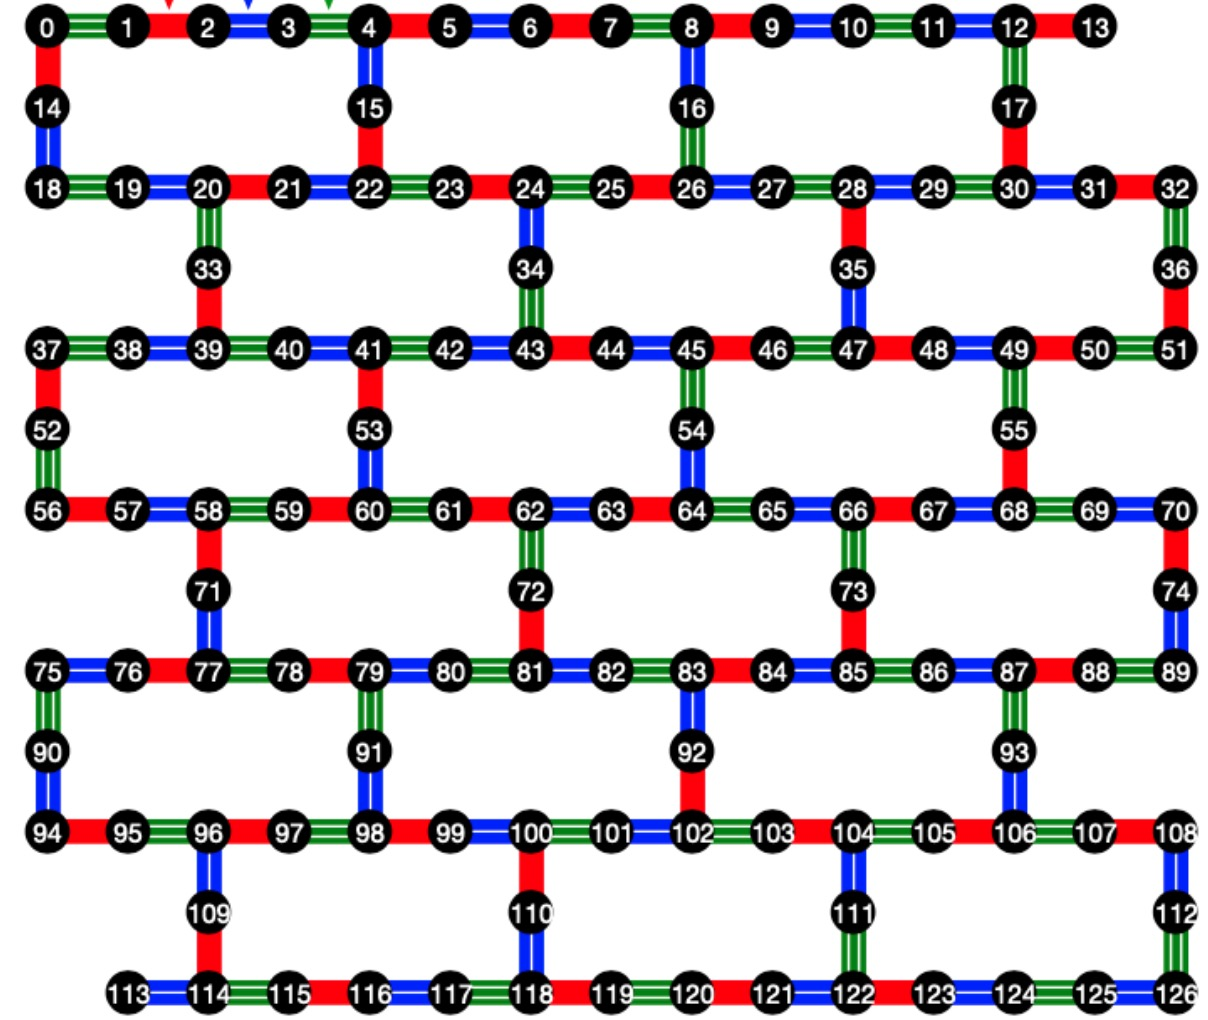
\includegraphics[width=\textwidth]{fig/ibm3.jpg}
  \end{figure}
   \end{minipage}
 
   %\textbf{Simulation Capabilities:}
   %   \begin{itemize}
    %  \item Can simulate mitigated results.
     % \item Cannot simulate noisy unmitigated results.
      %\end{itemize}
\end{frame}
\note{
  The IBM quantum computer is a typical NISQ device.

  Except for the noise, there is another factor that effects the quantum advantage. That is limitation of the locality of the gates.
  
As the right figure shows. This is the layout of IBM's quantum computer.

The black points represent the qubits, and the color lines represent the gates between the qubits.

The qubits can only interact with their nearest(near-st) neighbors(nei-bors), which causes the low entanglement entropy.

And the low entanglement entropy leads to the efficiency of the tensor network based simulation methods.


  A series(\textipa{'siri:z}) of works use improved(\textipa{im'pru:vd}) tensor network based simulation methods to successfully simulate the quantum expriment.

  But they can only complete the noiseless simulation, and can not simulate the noisy raw experimental data.
}

  \begin{frame}
  \cite{anand2023classical}\footcite{anand2023classical} proposed an improved experimental setting, which is more challenging for tensor network based simulation methods. 
    \begin{figure}
      \centering
    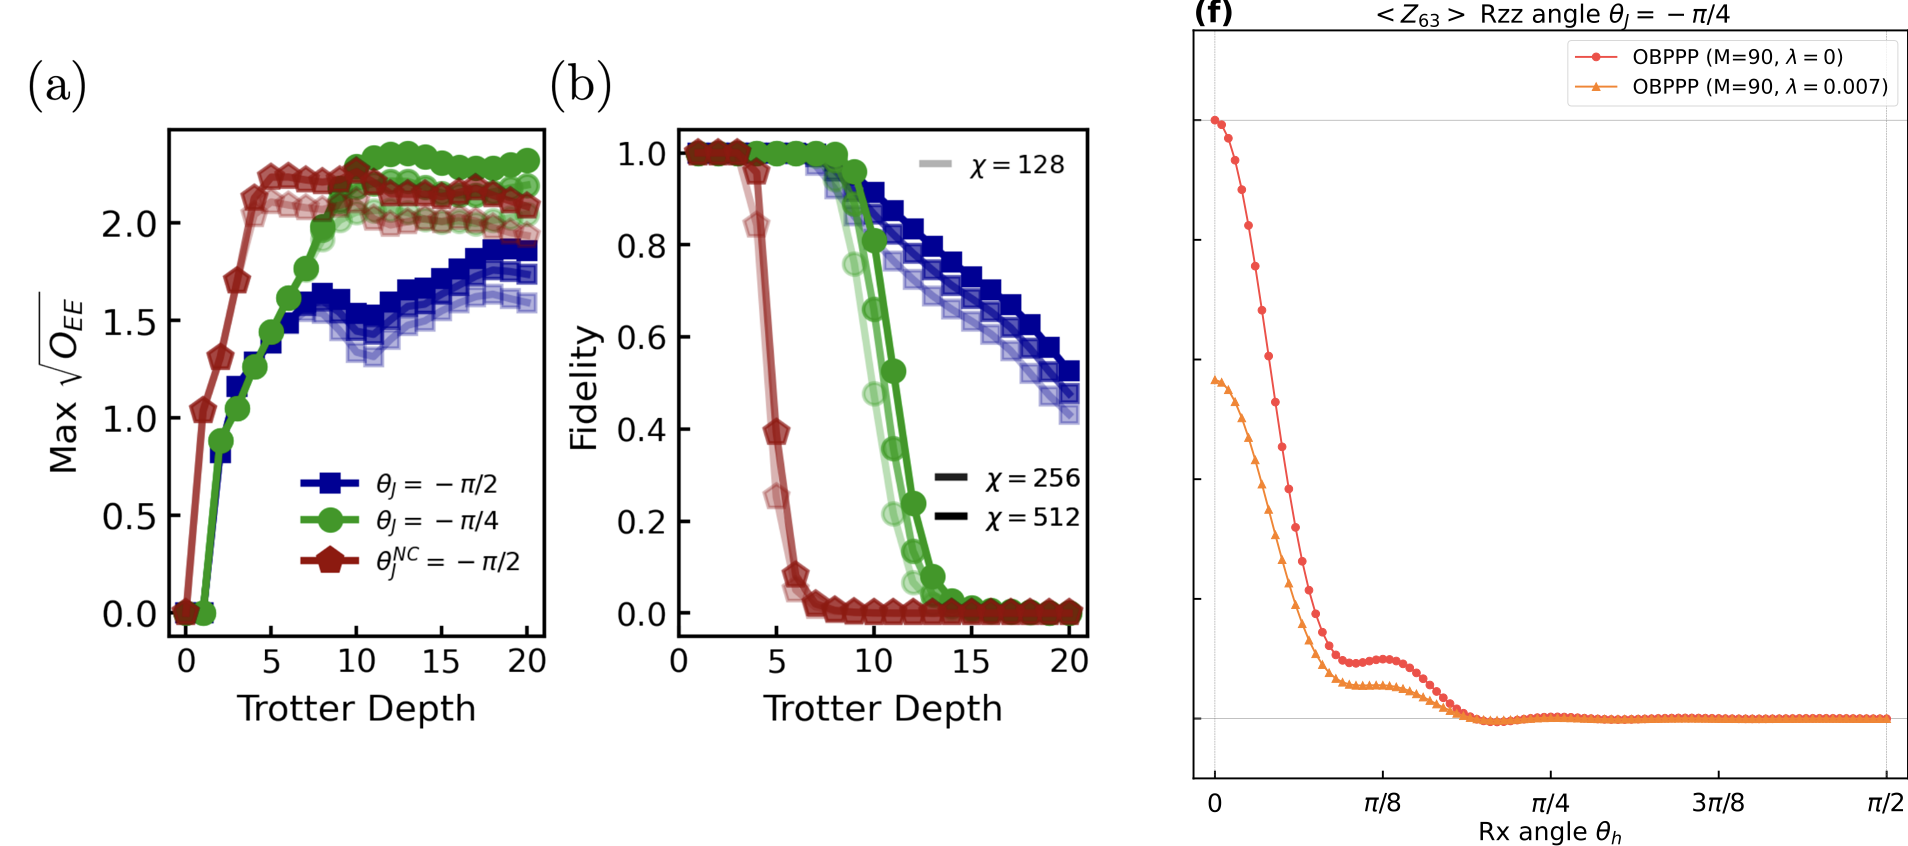
\includegraphics[width=\textwidth]{fig/simibm3.png}
    \end{figure}
  \begin{itemize}
    \item Theoretical prediction of mitigated results and noisy unmitigated results. \footnote{\textcolor{red}{Red line}: Theoretical prediction of mitigated results. \\
    \textcolor{orange}{Orange line}: Theoretical prediction of noisy unmitigated results.}
    \item Noise rate (0.007) is estimated from previously experimental data.
  \end{itemize}
  \vspace{1em}
\end{frame}
\note{
 To enhance the difficulty(\textipa{ˈdifikəlti}) of the simulation, an improved experimental setting is proposed. In this setting, the rotation angles of two-qubit gates in the quantum circuits are replaced(re-place-ed). 

 As the left figure shows, the original setting is labeled by the blue line, and the improved setting is labeled by the red line.

 As the circuit depth increases, the entanglement entropy of the improved setting grows faster than the original setting, which makes the tensor-network based simulation more challenging.

 The middle figure shows the fidelity which indicates the accuracy of the tensor network methods, higher is better. In the new setting, the fidelity decreases faster than the original setting, which means the simulation results are less accurate.

 But our method don't rely on the locality of the gates and low entanglement entropy, and it can still simulate the quantum circuits efficiently.

 Even no expriments for reference, we proposed a theoretical(\textipa{θiə'retik(ə)l}) prediction of the mitigated results and the noisy unmitigated results as the right figure shows.

 The unmitigated results are obtained by using the estimated noise rate from fiting the previously three figures, which is 0.007.
}


\begin{frame}[fragile]
  \begin{figure}
    \centering
    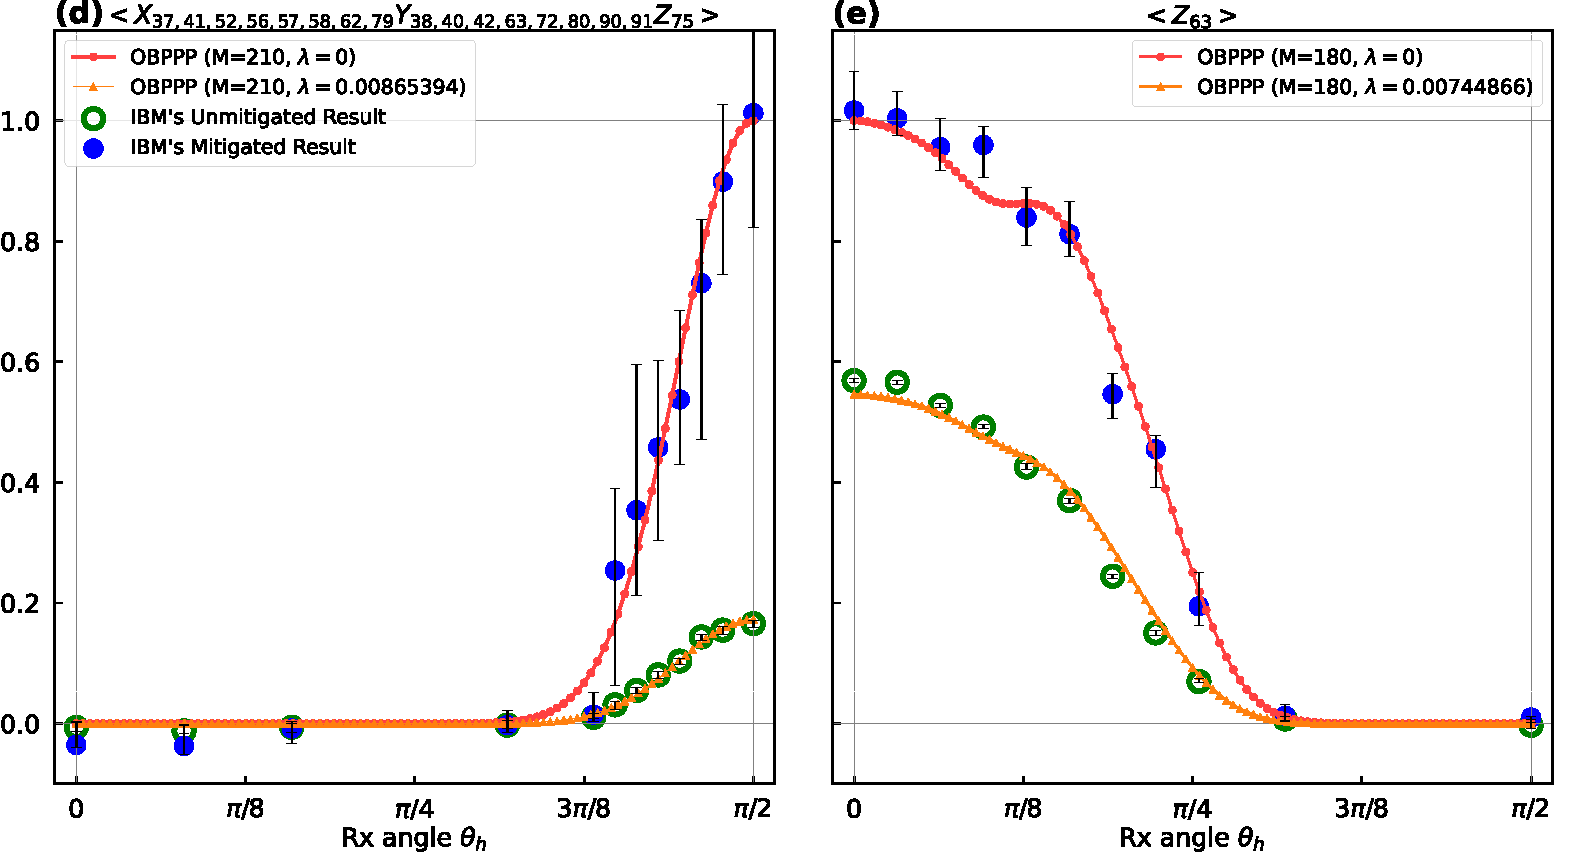
\includegraphics[width=\textwidth]{fig/simibm2.pdf}
  \end{figure}
  \begin{itemize}
    \item \textbf{No Exact References Available:} For deeper circuits, exact results are not available for comparison.
    \item \textbf{Simulation Consistency:}
    \begin{itemize}
        \item Noisy simulation results (\textcolor{orange}{orange}) align closely with noisy unmitigated results (\textcolor{green}{green points}).
  \end{itemize}
    \footnote{Runtime: 137s and 262s.}
\end{itemize}

\end{frame}
\note{For the last two figures in IBM experiments,
because there are too many qubits involved, there are no exact results for reference.

Other classical simulation methods provide different results that are inconsistent with each other and with the quantum computer's outputs.

But it's hard to compare whose results are more accurate, because of the lack of reference.

 However, we can still simulate the direct outputs of quantum computer and
 observed that the simulation results drawn in the orange line are consistent with the unmitigated results, drawn in green points.

 The unique(\textipa{ju'ni:k}) ability of our method to perform noisy simulation validates(\textipa{'vælideits}) our method by comparing with the unmitigated results.

}



\begin{frame}[fragile]{Numerical Simulation for Non-locality Circuits}
  \cite{pagano2020quantum}\footcite{pagano2020quantum} used a 1D array of ions to perform a low-depth long-range Quantum Approximate Optimization Algorithm (QAOA).
  \begin{figure}
    \centering
    \begin{subfigure}[t]{0.9\textwidth}
      \vtop{\null\hbox{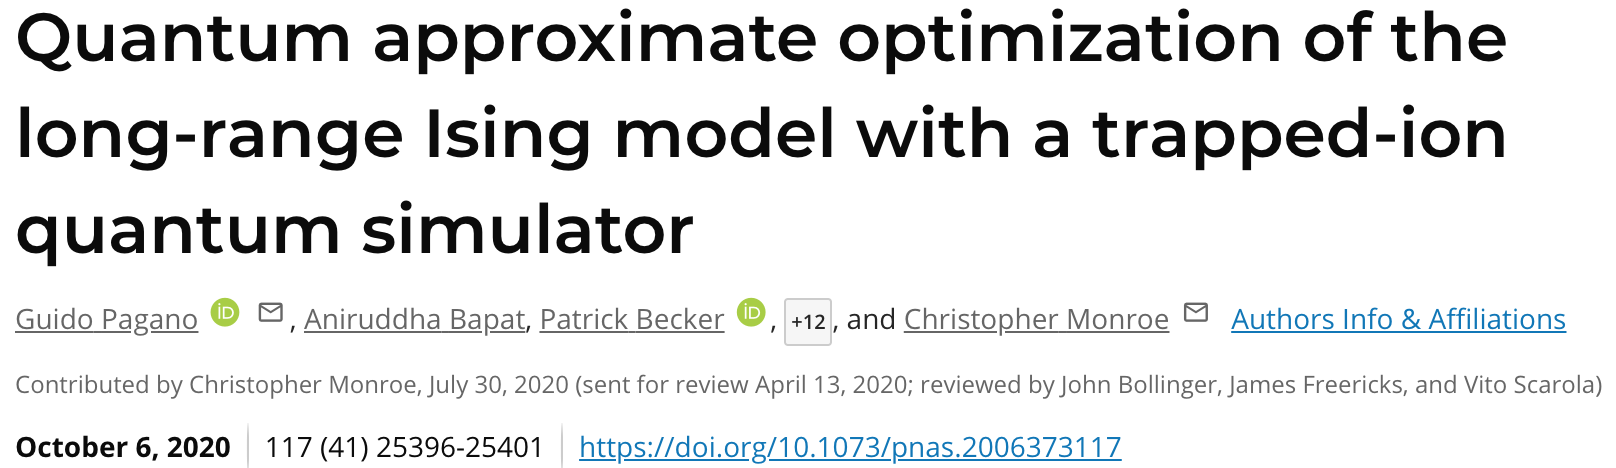
\includegraphics[width=\textwidth]{fig/ion1.png}}}
    \end{subfigure}
    \vfill
    \begin{subfigure}[t]{\textwidth}
      \begin{minipage}[t]{0.45\textwidth}
        \centering
        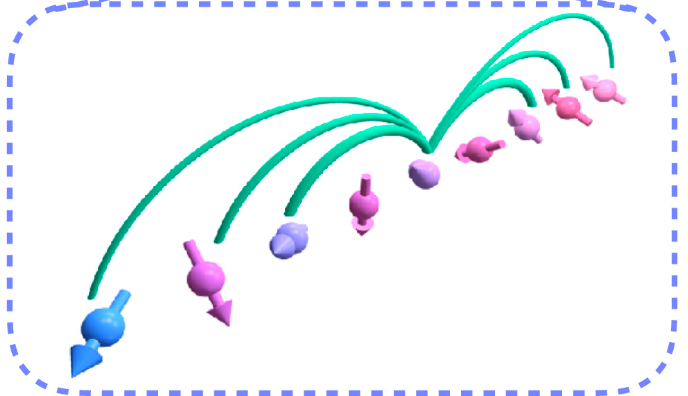
\includegraphics[width=\textwidth]{fig/ion2.png}
      \end{minipage}
      \hfill
      \begin{minipage}[t]{0.45\textwidth}
        \centering
        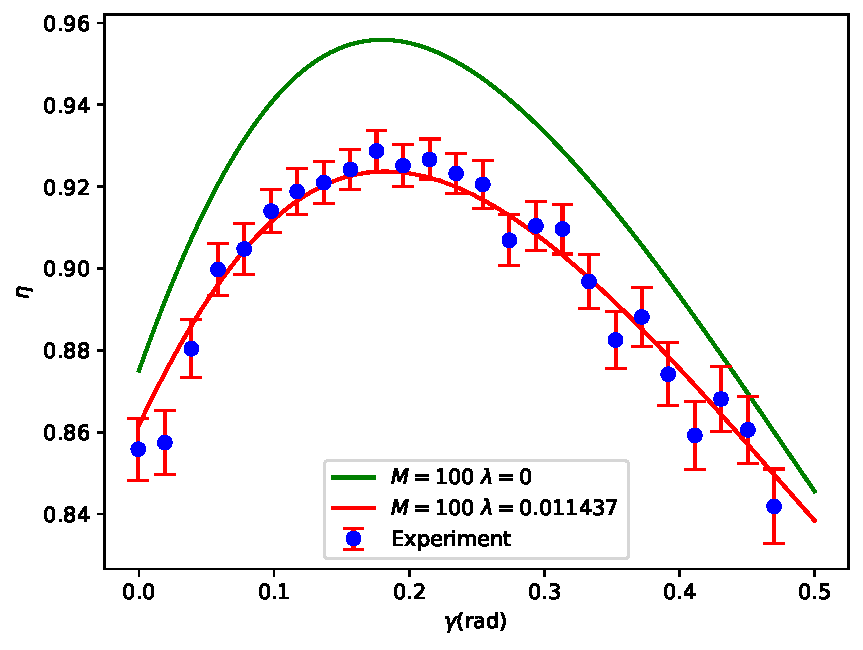
\includegraphics[width=\textwidth]{fig/QAOA.pdf}
      \end{minipage}
    \end{subfigure}
  \end{figure}
\end{frame}
\note{
  After we finished the simulation for IBM's experiments, we submitted our work to PRL. 
  During the review process, we recieved positive feedback from the referee.
  But one Referee asked the suitability (\textipa{ˈsuːtəb(ə)l}) of our method for different experiment platforms.

  To address this question, we apply our method to simulate an Ion Trap experiment, which use a 1D array of ions to run a low-depth long-range Quantum Approximate Optimization Algorithm (QAOA).

  The right figure shows the simulation results, 
  The red line is our noisy simulation results, and the blue points are the raw experimental data.
  We can see the simulation results are consistent with the experimental data.

}



\begin{frame}[fragile]{Theoretical Analysis}
  Not only practical utility, we also provide
  \vspace{-1em}
  \begin{itemize}
    \item A theoretical analysis of computational complexity.
    \item Error analysis of the simulation method.
    \item Rigorous proof of the polynomial scale cost.
  \end{itemize}
  
  \begin{mdframed}
For arbitrary $\varepsilon,\delta>0$ , the simulation ensures that the error is less than $\varepsilon$ with a probability of at least $1-\delta$. 
  
\textbf{Time Complexity:}
\vspace{-1em}
  \begin{itemize}
\item $\mathrm{Poly}(n) \order{L} \bigg(\frac{c}{\varepsilon \sqrt{\delta}} \bigg)^{\order{\sfrac{1}{\gamma}}}$ for Case 1
\item $\mathrm{Poly}(n)  \order{(nL)^{\frac{1}{2\gamma} \ln{\frac{c}{\varepsilon \sqrt{\delta}}}+1}}$ for Case 2
\end{itemize} 
    \end{mdframed}
    \begin{itemize}
      \item Considering current experimental capabilities, the cost scales \textcolor{red}{polynomially} with \(n\) and \(L\) in both cases\footnote{Here $n$ is the number of qubits, $L$ is the circuit depth, $c$ is a constant and $\gamma$ is a noise-related value.}.
      \item As noise vanishes (\(\gamma \to 0\)), the cost becomes uncontrolled due to the exponential dependency on \(\gamma^{-1}\).
  \end{itemize}
  

    %As noise vanishes (\(\gamma \to 0\)), the cost becomes uncontrolled due to the exponential dependency on \(\gamma^{-1}\).

    %When the noise vanishes, $\gamma$ approaches 0.
    \vspace{0.5em}
\end{frame}
\note{
  In addition to the practical utility, we also provide a theoretical analysis of the computational complexity of the simulation method.

  We analyze the error of the simulation method and rigorously prove that the cost is polynomial scale when the simulation error is bounded by a given threshold with high probability.

  The computational cost is shown in the box.
  For arbitrary epsilon and delta, the simulation ensures that the error is less than epsilon with probability at least 1 minus delta. With the cost is described in two cases.


  I will explain the two cases later. 

  For the both cases, the cost is polynomial scale to the number of qubits n and the circuit depth L. 

  And there is a exponent factor involves the noise-related value gamma.
  
  %For the first case, the computational cost is influenced by the noise related parameter gamma, and leads to a polynomial relationship with the number of qubits n and the circuit depth L.

  %For the second case, the n and L play a more intertwined(\textipa{ˌintɜ:'twaind}) role.

  %For the both cases, the cost is polynomial scale to n and L. And the exponent(\textipa{ik'spoʊnənt}) factor involves the noise-related gamma.
  
  As noise vanishes, the gamma approaches zero, the cost becomes uncontrolled due to the exponential dependency on the inverse of gamma.

  Thus our result didn't violate(\textipa{'vaiəleit}) the quantum complexity theory(\textipa{'θiəri}).

  This behavior aligns with quantum complexity theory, which suggests that the cost of simulating noiseless quantum circuits grows exponentially.
}





\begin{frame}[fragile]{Pauli Noise Model}
 Single-qubit Pauli noise model, which is defined as follows:
\begin{equation}\label{eq:single_qubit_noise}
\mathcal{N}(\phi)=(1-p_x-p_y-p_z)\phi+ p_x X\phi X+ p_y Y\phi Y+ p_z Z\phi Z,
\end{equation}
$p_x,p_y,p_z$ denote the \textcolor{red}{probabilities} of $X,Y,Z$ error occuring, respectively. 


\begin{figure}[tbp]
  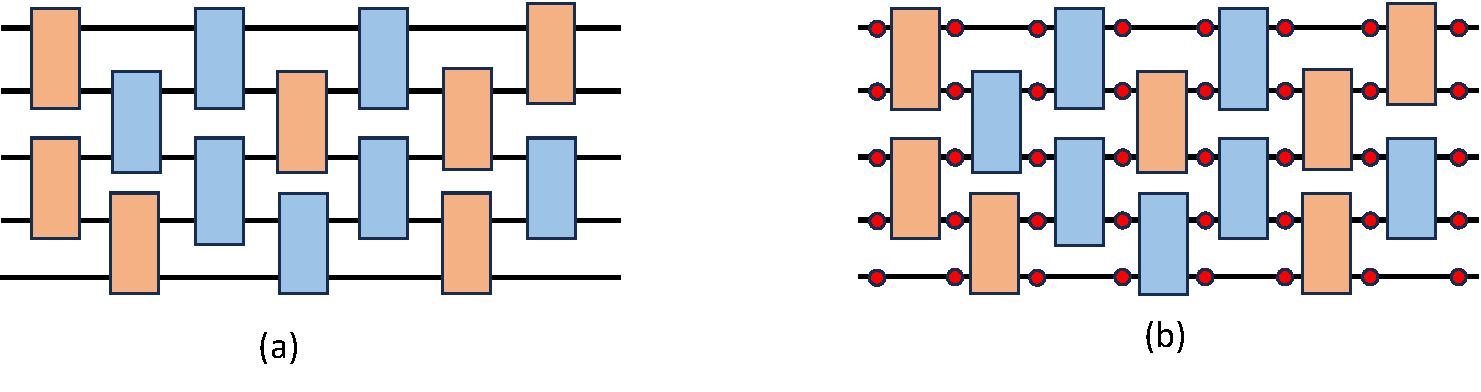
\includegraphics[width=240px]{fig/Circuit_comb.pdf}
\end{figure}
It is assumed that single-qubit Pauli noise $\mathcal{N}$ acts independently before each layer and the final observable.
\vspace{1em}
\footnotetext{
  \begin{itemize}
    \item Case 1: At least two non-zero elements in $\{p_x,p_y,p_z\}$.
    \item Case 2: Only one non-zero element in $\{p_x,p_y,p_z\}$.
  \end{itemize}
}
\end{frame}
\note{
Let me introduce the noise model.

 In our discussion, we consider the single-qubit Pauli noise model, which is defined as equation 1.

 This noise model is a probabilistic combination of the Pauli gates.

 The probabilities of the X, Y, and Z gates are p x, p y, and p z, respectively.


 As the figure shows, these red points represent the noise.

 It is assumed that the single-qubit Pauli noise acts independently before each layer and the final observable. 


 And the two cases I mentioned in the previous slide are defined by the noise model.

 If there are at least two non-zero elements in the probabilities, we call it Case 1.

 If there is only one non-zero element in the probabilities, we call it Case 2.
 % and they are applied throughout the quantum circuit.
}




\begin{frame}[fragile]{Pauli Path}
  \begin{mdframed}
    \textbf{A Pauli path}(\cite{aharonov2022polynomial}) for an \(L\)-layer circuit is a sequence: 
    \vspace{-1em}
    \begin{equation}
    s = (s_0, \dots, s_L) \in \bm{P}_n^{L+1},
    \text{where } \bm{P}_n = \Bigl\{\tfrac{\mathbb{I}}{\sqrt{2}}, \tfrac{X}{\sqrt{2}}, \tfrac{Y}{\sqrt{2}}, \tfrac{Z}{\sqrt{2}}\Bigr\}^{\otimes n} ,
    \vspace{-1em}
  \end{equation}
    \small{which describes the evolution path of the quantum state through the quantum circuit.}
  \end{mdframed}
  \vspace{-1em}
  \begin{figure}
    \centering
    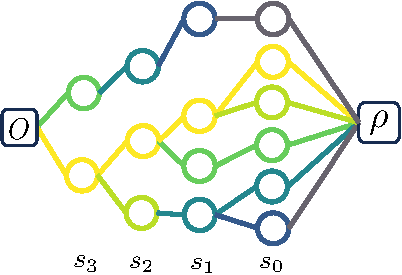
\includegraphics[width=0.3\textwidth]{fig/paulipath.pdf}
  \end{figure}
  \vspace{-1em}
 The observable value can be expressed as the sum (\textcolor{blue}{Fourier transform}):
  \begin{equation}
 \langle O \rangle=\sum_{s\in \bm{P}^{L+1}_n} f(\mathcal{U}(\bm{\theta}),s,O,\rho),
  \end{equation}
 where $f(\mathcal{U}(\bm{\theta}),s,O,\rho)$ denotes the contribution of a specific Pauli path $s=(s_0,\cdots,s_L)\in \bm{P}^{L+1}_n$:
 \vspace{-1em}
  \begin{equation}
 f(\mathcal{U}(\bm{\theta}),s,O,\rho)=\Tr{Os_L}\left(\prod_{i=1}^{L}\Tr{s_i\mathcal{U}_i s_{i-1}\mathcal{U}_i^\dagger}\right)\Tr{s_0\rho},
  \end{equation}
\end{frame}
\note{
 To simulate the observable value, we introduce the concept of the Pauli path.

 For a L layer ciruict, a Pauli path is a sequence of length L plus 1, represented as s=(s0 to sL) as the equation 2 shows.
 
 %in the set of all normalized n-qubit Pauli operators.

 \textbf{A Pauli path gives a specific evolution path of the quantum state through the quantum circuit.}

 The observable value can be expressed as the sum of contributions from all possible Pauli paths, as shown in equation 3.

 In this equation, the f term denotes the contribution of a specific Pauli path. And it can be calculated by equation 4.

 These equations transform the observable value into a sum of contributions from different path configurations. It can be viewed as a Fourier transform of the quantum circuit.
 }




\begin{frame}[fragile]{Truncated Pauli Paths}
  \vspace{-0.5em}
  When noise is present, contributions from Pauli paths are suppressed:\footnote{$\abs{s}_\mathcal{N}$ is noise-related Hamming weight.}
  \begin{equation}
  \begin{aligned}
      &\abs{\hat{f}(\mathcal{U}(\bm{\theta}),s,O,\rho)}\leq \textcolor{red}{\gamma^{\abs{s}_\mathcal{N}}} \abs{f(\mathcal{U}(\bm{\theta}),s,O,\rho)},\\
      &\text{where }  \gamma:=\min\{p|{p \in \{p_x,p_y,p_z\},p\neq 0}\} <1.
    \end{aligned}   
\end{equation}
    \vspace{-1em}
  \begin{figure}
    \centering
    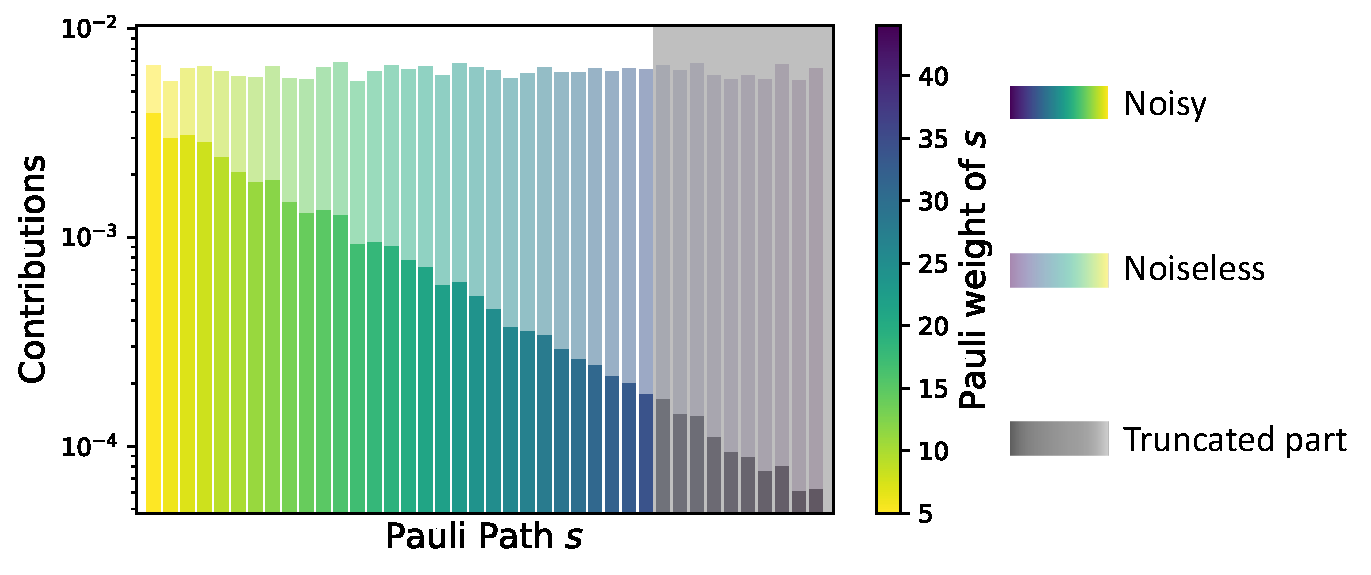
\includegraphics[width=0.7\textwidth]{fig/first.pdf}
  \end{figure}
  \vspace{-1em}
 This inspires calculates all contributions of the Pauli paths with $\abs{s}_\mathcal{N}\leq M$ to approximate ${\langle O \rangle}$:%\footnote{$M$ is a truncation parameter.} 
  \begin{equation}
 \widetilde{\langle O \rangle}:=\sum_{\textcolor{red}{\abs{s}_\mathcal{N}\leq M}} \hat{f}(\mathcal{U}(\bm{\theta}),s,O,\rho).
  \end{equation}
  Taking the \textcolor{blue}{low-order} terms of a Fourier-like expansion.
  \vspace{0.5em}
\end{frame}
\note{
  When noise is present, the contributions from Pauli paths are suppressed(\textipa{sə'prest}), as Equation 5 shows.

 The suppression(\textipa{sə'preʃ(ə)n}) factor is exponential to the noise-related Hamming weight of the Pauli path, and the gamma is less than 1.


 This inspires us to truncate the high-weight Pauli paths to approximate the noisy observable value. %Truncating the grey part and only calculating the left part.

 This is formalized as equation 6. The truncated noisy observable value is the sum of the contributions of all Pauli paths with the noise weight less than or equal to M.

 This approach can be viewed as taking the low-order terms of a Fourier-like expansion(ex-ban-sion), and truncating the higher-order contributions.

 In general case, the Fourier transform is taking in the function space, here we take it in the matrix algebra space.

 This is related to the field called Quantum Fourier Analysis(\textipa{ə'næləsis}). 

 And this brings an question, How to take the value of the truncation number M?

}
\begin{comment}
  \textcolor{red}{Jump}
 
  The noise effect on the Pauli path can be visualized as the figure shows.
  The x-axis(\textipa{'æksis}) represents the Pauli path, and the weight of the Pauli path increases from left to right.
 
  The y-axis represents the contribution of the Pauli path.
 
  The translucent bars represent noiseless contributions, while opaque bars show the contributions after noise.

  They are exponentially suppressed by the noise factors.

  \textcolor{red}{Jump}
  \end{comment}

\begin{frame}
  \begin{figure}
    \centering
    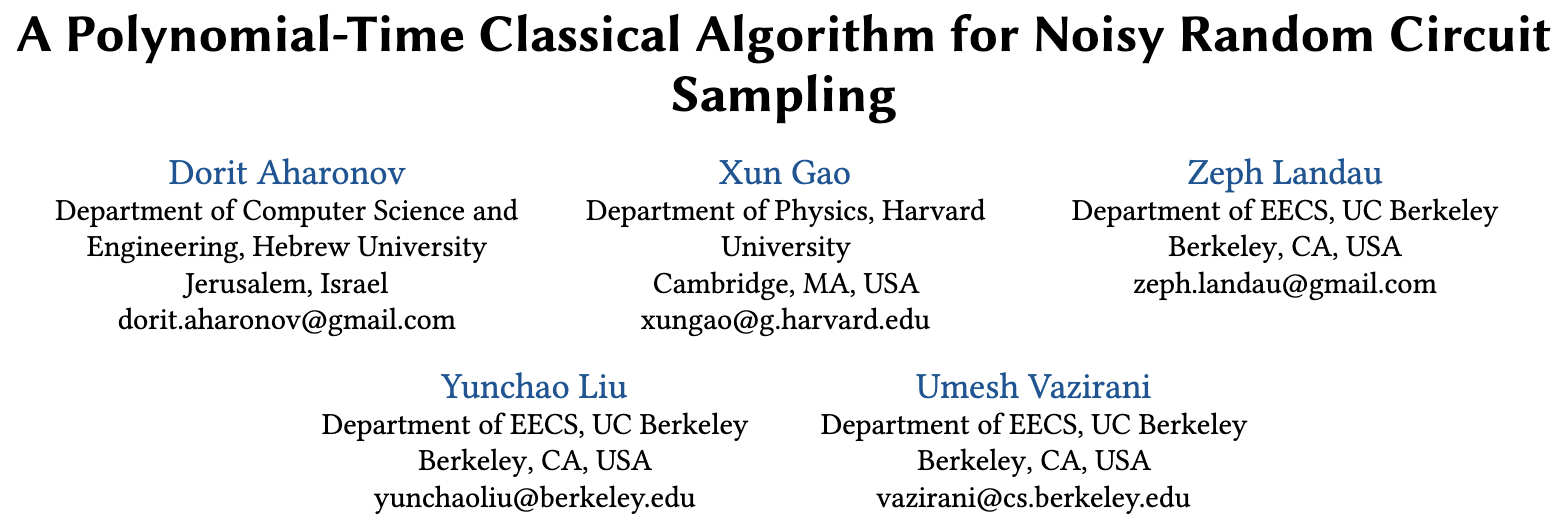
\includegraphics[width=\textwidth]{fig/gaoxun.png}
  \end{figure}
  The idea of the truncated Pauli path is inspired by the above wonderful work. Different in the noise model and the quantum circuits.
  \begin{itemize}
    \item \textbf{Their: Depolarizing noise + Random Circuit Sampling} (2-design).
    \item \textbf{Ours: Pauli-type noise + Typical parameterized quantum circuits} (Clifford gates + Rotation gates).
  \end{itemize}
  We also provide an efficient practical simulation method and conclude
the efficiency is due to the choices of noise model and quantum circuits.

Find a new ”easy island” in the ”hard ocean” of quantum circuits simulations.
\end{frame}
\note{
  The idea of the truncated Pauli path is inspired by the above wonderful work.
  
  This work rigorously proves the when depolarizing noise is present, classical simulation cost for random circuit sampling tasks is polynomial scale.

  Our work is different from theirs in the noise model and the quantum circuits.

  They consider the depolarizing noise and random circuit sampling, which is the 2-design ensemble.

  While we consider the Pauli-type noise and typical parameterized quantum circuits, which consist of Clifford gates and parameterized rotation gates.

  We also provide an efficient practical simulation method and conclude that the efficiency is due to the choices of the noise model and quantum circuits.

  Our work finds a new "easy island" in the "hard ocean" of quantum circuits simulations.
}

\begin{frame}{Error Analysis}
  \begin{mdframed}
  \begin{lemma}\label{lemma:MSE_l}
 Suppose the quantum circuit $\mathcal{U}(\bm{\theta})$ is splittable, for $\forall\nu > 0$, given \textcolor{blue}{$M\geq\frac{1}{4\gamma}\ln{\frac{\norm{O}_\infty^2}{\nu}}$}, where $\gamma:=\min\{p|{p \in \{p_x,p_y,p_z\},p\neq 0}\}$. Then \textbf{the mean-square error} $\mathbb{E}_{\bm{\theta}}\abs{\widetilde{\langle O \rangle}-\langle O \rangle}^2 \leq \nu$, where $\bm{\theta}$ satisfies uniformly distributed in $[0,2\pi]^{\sum_{i=1}^{L}R_i}$.
  \end{lemma}
  \end{mdframed}
\begin{itemize}
  \item $M$ is \textcolor{red}{independent} of the number of qubits $n$, the circuit depth $L$ and circuit construction.
\end{itemize}
\end{frame}
\note{
 The truncation error can be analyzed by the mean-square error.

 As the lemma shows, %assume the quantum circuit is splittable, 
 for any given precision nu, if the truncation number M is greater than or equal to the blue part. 
 Where the noise related value gamma is defined as the minimum of the non-zero noise probabilities.
 
 Then the mean-square error is less than nu.

 Here we can see that the truncation number M is independent of the number of qubits n, the circuit depth L and the circuit construction.
}

\begin{frame}{Observable's back-propagation on Pauli paths (OBPPP)}
  To calculate the sum of contributions from Pauli paths with \textcolor{red}{\(\abs{s}_\mathcal{N} \leq M\)}, we propose the OBPPP algorithm. %and calculate the truncated exception value $\widetilde{\langle O \rangle}$. The 
  \begin{figure}
    \centering
    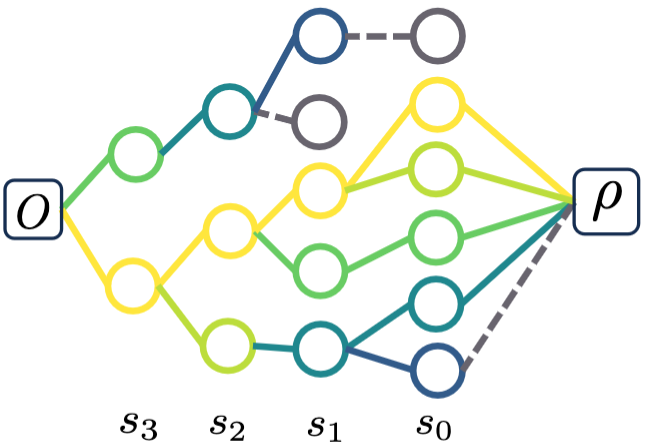
\includegraphics[width=0.4\textwidth]{fig/obppp.png}
  \end{figure}
  \begin{mdframed}
 The time complexity of OBPPP is 
 \begin{itemize}
 \item $\mathrm{Poly}(n)\order{L}\textcolor{red}{2^M}$ for Case 1
 \item $\mathrm{Poly}(n)\order{\textcolor{red}{(nL)^{M+1}}}$ for Case 2
 \end{itemize} %The space complexity in both scenarios is $\order{\mathrm{Poly}(n)+nL}$.
\end{mdframed}
\vspace{0em}
\footnotetext{
  \begin{itemize}
    \item Case 1: At least two non-zero elements in $\{p_x,p_y,p_z\}$.
    \item Case 2: Only one element in $\{p_x,p_y,p_z\}$ non-zero.
  \end{itemize}
  $n$ : number of qubits, $L$ : number of layers.
}
\end{frame}
\note{
 To calculate the truncated sum of Pauli path, we propose the observable's back-propagation(\textipa{prɒpə'geiʃn}) on Pauli paths algorithm.

 As showing in the figure, the algorithm starts from the observable operator O and back-propagate(\textipa{'prɒpəgeit}) through the circuit from the final layer to the initial layer.


 During the back-propagation, the algorithm discards(\textipa{di'ska:rdz}) paths with weight greater than M.

 As the computation cost. %Assume the observable operator O and the input state rho are sparse, which is a common assumption, otherwise, the quantum circuit configurations can't be input into the classical computer.

 The time complexity of the OBPPP algorithm is divided into two cases.
 The cases are dependent on the number of non-zero elements in the noise probabilities.
 
 For the both cases, the time complexity is polynomial in the number of qubits n, the circuit depth L, and exponential to truncation number M.

 Combing the computational cost and error analysis, we can get the main result of our work.
 
 %for case 1. %The case is when at least two non-zero elements in the noise probabilities.

 %While for case 2, %the case when only one non-zero element in the noise probabilities, 
 %the time complexity is n product L to the power of M plus 1.

 %In the following, I will show that for a given precision(pre-ci-sion) and noise rate, the truncation number is independent to n and L. Thus leading to the polynomial time complexity.

}

\begin{comment}
  \begin{mdframed}
    \begin{definition}
 For a $2^n$ dimension Hilbert space $\mathcal{H}$, a density operator $\rho\in \langle O \rangle(\mathcal{H})$ is sparse if the number of non-zero elements is polynomially related to the number of qubits $n$, formulated as $\abs{\{\rho_{i,j}|\rho_{i,j}\neq 0 \text{ for }i,j=1,\cdots 2^n\}}=\order{\mathrm{Poly}(n)}$. 
    \end{definition}
    \begin{definition}
 For a $2^n$ dimension Hilbert space $\mathcal{H}$,
 an observable operator $O\in \langle O \rangle(\mathcal{H})$ is termed pauli-sparse if its Pauli decomposition $O=\sum_{\sigma}c_{\sigma}\sigma$, where $\sigma\in\{\mathbb{I},X,Y,Z\}^{\otimes n}$, satisfies the condition that the number of non-zero coefficients $\abs{\{c_{\sigma}|c_{\sigma}\neq 0 \}}=\order{\mathrm{Poly}(n)}$.
    \end{definition}
  \end{mdframed}
\end{comment}


\begin{frame}[fragile]{Main Results}

\begin{mdframed}
\begin{theorem}\label{thm:main}
 Suppose the quantum circuit $\mathcal{U}(\bm{\theta})$ is splittable and $O,\rho$ are (pauli-)sparse. For a fixed $\gamma:=\min\{p|{p \in \{p_x,p_y,p_z\},p\neq 0}\}$ and arbitrary truncation error $\varepsilon$, there exists a classical algorithm to determine the truncated noisy observable value $\widetilde{\langle O \rangle}$. This value satisfies $\abs{\widetilde{\langle O \rangle}-\langle O \rangle} \leq \varepsilon$ with a probability of at least $1-\delta$ over a uniform distribution of $\bm{\theta}\in [0,2\pi]^{\sum_{i=1}^{L}R_i}$. 
 
 The time complexity is 
 \begin{itemize}
 \item $\mathrm{Poly}(n) \order{L} \bigg(\frac{\norm{O}_\infty}{\varepsilon \sqrt{\delta}} \bigg)^{\order{\sfrac{1}{\gamma}}}$ for Case 1
 \item $\mathrm{Poly}(n)  \order{(nL)^{\frac{1}{2\gamma} \ln{\frac{\norm{O}_\infty}{\varepsilon \sqrt{\delta}}}+1}}$ for Case 2.
 \end{itemize}
\end{theorem}
\end{mdframed}
\vspace{0em}
\footnotetext{
  \vspace{-1.5em}
  \begin{itemize}
    \item Case 1: At least two non-zero elements in $\{p_x,p_y,p_z\}$.
    \item Case 2: Only one element in $\{p_x,p_y,p_z\}$ non-zero.
  \end{itemize}
  $O$ is the observable operator, $\bm{\theta}$ is the rotation angles, $n$ is the number of qubits, $L$ is the circuit depth.
}
\end{frame}
\note{

 For a fixed noise rate gamma which is defined as the minimum of the non-zero noise probabilities, and the arbitrary error epsilon, there exists a classical algorithm to determine(deter-min) the truncated noisy observable value. And the error of the estimation is less than epsilon with the success probability of at least 1 minus delta. over a uniform distribution of the rotation angles.

 And the time complexity is polynomial scale.
}



\begin{frame}
  \begin{mdframed}
  \begin{corollary}
    \label{prop:lambda_and_L}
 For depolarizing noise, assume the quantum circuit $\mathcal{U}(\bm{\theta})$ is splittable and both $O,\rho$ are (pauli-)sparse, with $\norm{O}_\infty$ fixed.
 To estimate $\widetilde{\langle O \rangle}$ with $\mathbb{E}_{\bm{\theta}}\abs{\widetilde{\langle O \rangle}-\langle O \rangle}^2$ less than a sufficiently small constant,
 we have 
      
 1. If \textcolor{red}{$\gamma=\Omega(\frac{1}{\log{L}})$}, a classical algorithm exists that can simulate the circuit in time $\mathrm{Poly}\left(n,L\right)$. 
      
 2. If \textcolor{blue}{$\gamma=\order{\frac{1}{L}}$}, there are instances where OBPPP method exhibits exponential time complexity with respect to $L$.
  \end{corollary}
  \end{mdframed}

  \begin{itemize}
    \item $\gamma$ is essential to keep below \textcolor{green}{$o(\frac{1}{\log L})$} to ensure the quantum circuit simulation is hard.
  \end{itemize}
\end{frame}
\note{
 For the depolarizing noise, we can get the corollary(ke-ro-leri;\textipa{kə'rɒləri}).

 If the experiment is improved, the noise would be reduced. So we can increase the circuit depth to do more computation.


 This result shows a relationship between the noise rate gamma and the circuit depth L.

 If the noise rate gamma is at least inverse logarithmic(log-raise-mic;\textipa{ˌlogə'riðmik}) in the circuit depth L, our classical algorithm can still complete the computation in polynomial time.

 While if the noise rate gamma is at most inverse of the circuit depth L, there are instances that our method would exhibits(\textipa{ig'zibits}) exponential time to L.

 This corollary shows that the noise rate gamma is essential to keep below inverse logarithmic(log-raise-mic) in the circuit depth L to ensure the quantum circuit simulation is hard.
}


\section{Simulating noiseless near-Clifford circuits}
\begin{frame}[fragile]
  Can we use the Pauli path integral method to simulate the ideal \textcolor{red}{noiseless} quanrum circuits?

  \fullcite{zhang2024clifford}


   \begin{itemize}
     \item \textbf{Simulation Method:} A method to simulate the noiseless observable value of near-Clifford circuits (small angle space): Sparse Pauli Dynamics~(SPD)~\footcite{beguvsic2024fast}.
     \item \textbf{Application:} The near-Clifford circuits noiseless simulation results can be used to mitigate the noise in real quantum experiments.
     %\item Provide a theoretical analysis of the quantum advantage in noisy variational quantum algorithms.
     %\item Develop a high-performance program to implement the simulation method and apply it to simulate IBM's 127-qubit experiment.
   \end{itemize}
 \end{frame}

 \begin{frame}[fragile]{Pauli Path Integral For Noiseless Circuits}
  When the rotation parameters are located in the small angle space $\Theta=\{\bm{\theta}\mid \abs{\theta_i}\leq \theta_* ,i=1,\cdots,L \}$, the truncation error can be upper bounded, as summarized in the following theorem. 
  \begin{mdframed}
    \begin{theorem}\label{thm:truncation_error}
      For any given $\delta>0$, $M>0$ satisfies $\frac{\ln{1+\frac{\delta}{2}}}{L-M}\leq \frac{\ln{2}}{M}$, and Pauli observable $O$:
    \begin{itemize}
      \item If $\theta_*=\frac{\ln{1+\frac{\delta}{2}}}{L-M}=\order{\frac{1}{L-M}}$, then the truncation error satisfies $\abs{\langle O \rangle - \langle O \rangle ^{(M)}}\leq \delta$ for all $\bm{\theta}\in \Theta$.
      \item In average case, if $\theta_*=\sqrt{\frac{3\ln{1+\frac{\delta}{2}}}{L-M}}=\order{\frac{1}{\sqrt{L-M}}}$, then the mean square error $\mathbb{E}_{\bm{\theta}\in \Theta}[(\langle O \rangle - \langle O \rangle ^{(M)})^2]\leq \delta$.
    \end{itemize} 
    \end{theorem}
  \end{mdframed}
  \vspace{0em}
  \footnotetext{
    %\vspace{-1.5em}
    $O$ is the observable operator, $\bm{\theta}$ is the rotation angles, $n$ is the number of qubits, $L$ is the circuit depth.
  }
\end{frame}

\begin{frame}[fragile]{Application in Quantum Error Mitigation}
  Clifford Perturbation Data Regression (CPDR) 
  \begin{figure}
    \centering
    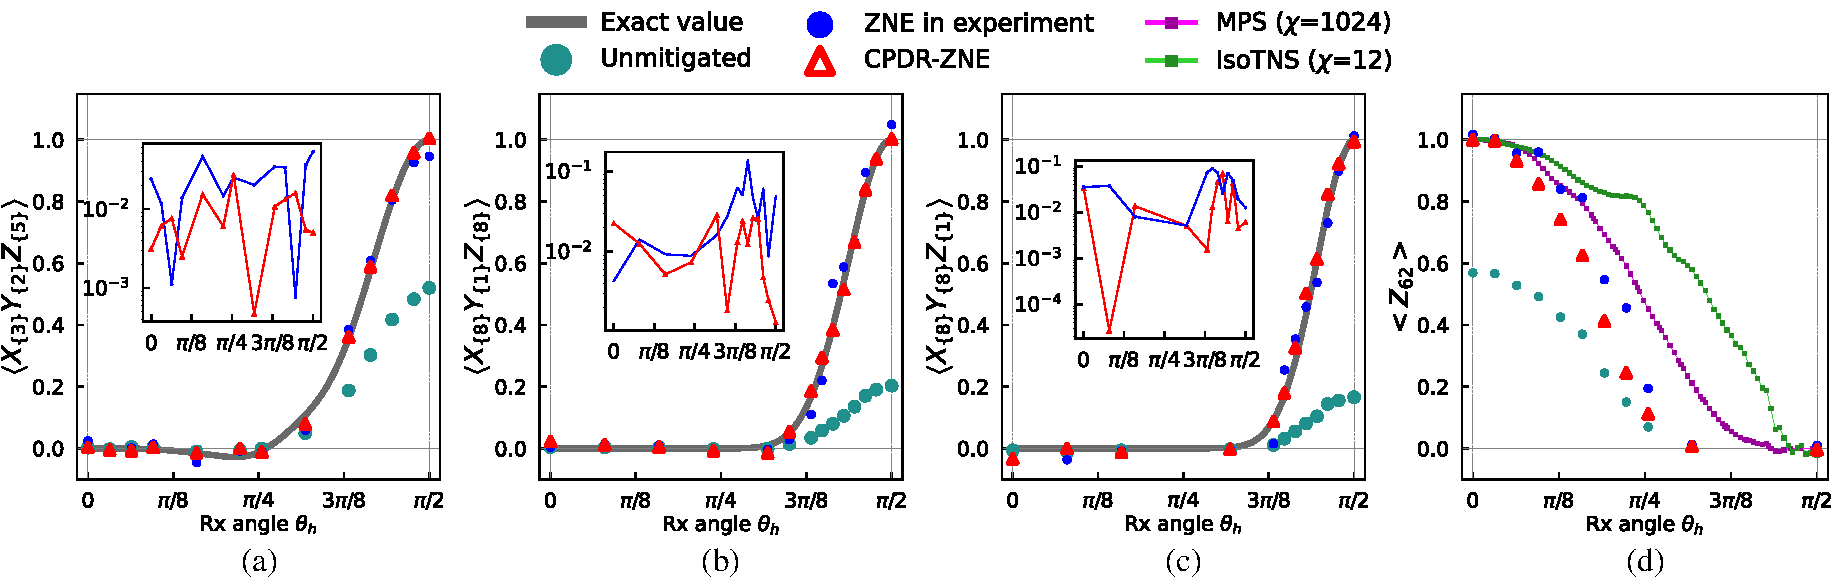
\includegraphics[width=\textwidth]{fig/IBM_ans_v4.pdf}
  \end{figure}
\end{frame}


\section{Conclusion}

\begin{frame}[fragile]{Summary}
  \begin{itemize}
    \item We propose a polynomial-scale classical algorithm to simulate the observable value of the noisy quantum circuits.
    \item  Containing most variational quantum algorithms.
    \item The efficiency of the algorithm is verified by IBM's 127-qubit experiments, and can be used to fit the raw experimental data.
    \item The algorithm is also efficient for the improved experimental setting proposed by \cite{anand2023classical}.
    \item The efficiency of the algorithm is irrelevant to the locality of the gates and the entanglement entropy. 
    \item For noiseless circuits, Pauli path integral method can also be used to simulate the noiseless observable value of near-Clifford circuits.
  \end{itemize}
\end{frame}
\note{
  In summary, we propose a polynomial-scale classical algorithm to simulate the observable value of the noisy quantum circuits.

  This contains most variational quantum algorithms.

  The efficiency of the algorithm is verified by IBM's 127-qubit experiments, and can be used to fit the raw experimental data.

  The algorithm is also efficient for the improved experimental setting proposed by \cite{anand2023classical}.

  And the efficiency of our algorithm is irrelevant(i-relevant) to the locality of the gates and the entanglement entropy.
}


\begin{frame}[fragile]{Future Work}
  \begin{itemize}
    \item Consider other circuit ensembles~(local scrabling) and noise models~(non-unital).
    \item Combing with tensor network~(stablizer tensor network).
    \item Find noise bottleneck in quantum circuits.
    \item Worst-case analysis, noise threshold, monte-carlo method?
  \end{itemize}
\end{frame}
\note{
  For the future work, we plan to consider other circuit ensembles and noise models.

  For example, the local scrambling circuit ensemble and the non-unital noise model.

  We also plan to combine our method with tensor network methods, such as the stabilizer tensor network.

  And we can use this method to find the noise bottleneck in the quantum circuits.

  Given a structure of the quantum circuit, we try to find the position where the noise has the most significant impact.

  We also plan to do the worst-case analysis, maybe in worst-case, the noise threshold is important. And maybe monte-carlo method can be used to improve the efficiency of the simulation. 
}

\begin{frame}[standout]
 Thank you\\
\end{frame}
\note{
  %Thank the ICCM committee for giving me the opportunity to present my work. It's a great honor to be nominated for the Graduate Thesis(\textipa{θi:sis}) Award.
  %And thank you for your attention!

  I would like to express my gratitude(gra-ti-tude) to the ICCM committee for giving me the opportunity to present my work. 
  
  It’s truly an honor for me to recieve the Graduate Thesis(\textipa{'θi:sis};see-se-si) Award(a-war-d).

  Thank you to everyone for your attention and interest in my research. 

  And thank the organizer for the opportunity to give me a chance to communicate with you.

  I appreciate the chance to share my findings with you today!
}
\appendix

\begin{frame}[fragile]{Backup slides}
 Sometimes, it is useful to add slides at the end of your presentation to
 refer to during audience questions.

 The best way to do this is to include the \verb|appendixnumberbeamer|
 package in your preamble and call \verb|\appendix| before your backup slides.

  \themename will automatically turn off slide numbering and progress bars for
 slides in the appendix.%新方法,新的资源 利用噪声和Clifford结果
\end{frame}

%\begin{frame}[allowframebreaks]{References}

  %\bibliography{../aps_preprint}
  %\bibliographystyle{abbrv}

%\end{frame}
\end{CJK}
\end{document}